\documentclass[12pt,onesided]{amsart} 

%%%%%%%%%%%%%%%%%%%%%%%%%%%%%%%%%%%%%%%%%%%%%%%%%%
%%%%%%%%%%%%%%%%%%%% PREAMBLE %%%%%%%%%%%%%%%%%%%%
%%%%%%%%%%%%%%%%%%%%%%%%%%%%%%%%%%%%%%%%%%%%%%%%%%


% -------------------- defaults -------------------- %
% load lots o' packages

% layout control
\usepackage{geometry}
\geometry{verbose,tmargin=1.25in,bmargin=1.25in,lmargin=1.1in,rmargin=1.1in}
\usepackage{parallel}
\usepackage{parcolumns}
\usepackage{fancyhdr}

% math typesetting
\usepackage{array}
\usepackage{amsmath}
\usepackage{amssymb}
\usepackage{amsfonts}
\usepackage{relsize}
\usepackage{mathtools}

% restricts float objects to be inserted before end of section
% creates float barriers
\usepackage[section]{placeins}

% tables
\usepackage{tabularx}
\usepackage{booktabs}
\usepackage{multicol}
\usepackage{multirow}
\usepackage{longtable}

\usepackage[%
decimalsymbol=.,
digitsep=fullstop
]{siunitx}

% to adapt caption style
\usepackage[font={small},labelfont=bf]{caption}

% references
\usepackage{natbib}

% footnotes at bottom
\usepackage[bottom]{footmisc}

% to change enumeration symbols begin{enumerate}[(a)]
\usepackage{enumerate}

% to make enumerations and itemizations within paragraphs or
% lines. f.i. begin{inparaenum} for (a) is (b) and (c)
\usepackage{paralist}

% to colorize links in document. See color specification below
\usepackage[pdftex,hyperref,x11names]{xcolor}

% for multiple references and insertion of the word "figure" or "table"
% \usepackage{cleveref}

% load the hyper-references package and set document info
\usepackage[pdftex]{hyperref}

% graphics stuff
\usepackage{subfig}
\usepackage{graphicx}
\usepackage[space]{grffile} % allows us to specify directories that have spaces
\usepackage{placeins} % prevents floats from moving past a \FloatBarrier
\usepackage{tikz}

% \usepackage[figuresright]{rotating}
% \newenvironment{amssidewaysfigure}  {\begin{sidewaysfigure}\vspace*{.8\textwidth}\begin{minipage}{\textheight}\centering}
%   {\end{minipage}\end{sidewaysfigure}}

\usepackage{rotating}

% Spacing
\usepackage[doublespacing]{setspace}

% define clickable links and their colors
\hypersetup{%
	unicode=false,          % non-Latin characters in Acrobat's bookmarks
	pdftoolbar=true,        % show Acrobat's toolbar?
	pdfmenubar=true,        % show Acrobat's menu?
	pdffitwindow=false,     % window fit to page when opened
	pdfstartview={FitH},    % fits the width of the page to the window
	pdfnewwindow=true,%
	pagebackref=false,%
	pdfauthor={Shahryar Minhas},%
	pdftitle={Let's say Amen for Latent Space Models},%
	colorlinks,%
	citecolor=black,%
	filecolor=black,%
	linkcolor=black,%
	urlcolor=RoyalBlue4
}

% Fonts
\usepackage[default,osfigures,scale=0.95]{opensans}
\usepackage[T1]{fontenc}
\usepackage{ae}

% Generate some fake text
\usepackage{blindtext}

% -------------------------------------------------- %


% -------------------- title -------------------- %

\title{Let's say Amen for Latent Space Models}
\vspace{\baselineskip}

\author[Minhas]{Shahryar Minhas}
\address{Shahryar Minhas: Department of Political Science}
\curraddr{Michigan State University}
\email{s7.minhas@gmail.com}

\author[Hoff]{Peter D. Hoff}
\address{Peter D. Hoff: Department of Statistics}
\curraddr{Duke University}
\email{pdhoff@duke.edu}

\author[Ward]{Michael D. Ward}
\address{Michael D. Ward: Department of Political Science}
\curraddr{Duke University}
\email{michael.d.ward@duke.edu}

\date{\today}

\setlength{\headheight}{15pt}
\setlength{\headsep}{20pt}
\pagestyle{fancyplain}
 
\fancyhf{}
 
\lhead{\fancyplain{}{}}
\chead{\fancyplain{}{Amen for LSM}}
\rhead{\fancyplain{}{\today}}
\rfoot{\fancyplain{}{\thepage}}

% ----------------------------------------------- %


% -------------------- customizations -------------------- %

% references to graphics
\makeatletter
\def\input@path{{/Users/janus829/Dropbox/Research/netModels/summResults/}, {/Users/s7m/Dropbox/Research/netModels/summResults/}}
\makeatother
\graphicspath{{/Users/janus829/Dropbox/Research/netModels/summResults/}, {/Users/s7m/Dropbox/Research/netModels/summResults/}}

% easy commands for number propers
\newcommand{\first}{$1^{\text{st}}$}
\newcommand{\second}{$2^{\text{nd}}$}
\newcommand{\third}{$3^{\text{rd}}$}
\newcommand{\nth}[1]{${#1}^{\text{th}}$}

% easy command for boldface math symbols
\newcommand{\mbs}[1]{\boldsymbol{#1}}

% command for R package font
\newcommand{\pkg}[1]{{\fontseries{b}\selectfont #1}}

% approx iid
\newcommand\simiid{\stackrel{\mathclap{\normalfont\mbox{\tiny{iid}}}}{\sim}}

% -------------------------------------------------------- %

%%%%%%%%%%%%%%%%%%%%%%%%%%%%%%%%%%%%%%%%%%%%%%%%%%
%%%%%%%%%%%%%%%%%%%% DOCUMENT %%%%%%%%%%%%%%%%%%%%
%%%%%%%%%%%%%%%%%%%%%%%%%%%%%%%%%%%%%%%%%%%%%%%%%%

\begin{document}
\maketitle\thispagestyle{empty}

\begin{quote}
\small{\singlespacing{There is growing interest in the study of political networks. Network analysis allows scholars to move away from focusing on individual observations to the interrelationships among observations. Many network approaches have been developed in descriptive fashion, and until recently most network studies have been descriptive. However, with greater interest in networks inferential work with networks has been growing. We review a new approach that models interdependencies among observation using additive and multiplicative effects, this approach can be applied to binary, ordinal, and continuous network data. In addition this approach, called AME, provides a set of tools for inference on longitudinal networks as well. We develop this approach and compare it to those examined in the recent survey by Cranmer et al. (2016).  The AME approach is shown to be a) easy to implement, b) interpretable in a general linear model framework, c) computationally straightforward, d) is not prone to degeneracy, e) captures 1st, 2nd, and 3rd order network dependencies, and f) notably outperforms multiple regression quadratic assignment procedures, exponential random graph models, and latent space approaches using Euclidean distance metrics on a variety of metrics. AME offers a straightforward way to undertake nuanced, principled inferential network analysis for a wide range of social science questions. 

% overview
% We introduce the Additive and Multiplicative Effects (AME) modeling framework for studying network data and show that it provides superior performance in terms of capturing network dependencies and overall performance to existing alternatives. }}
\end{quote}

\newpage\setcounter{page}{1} 

Network analysis provides a way to represent and study ``relational data'', that is data with characteristics extending beyond those of the individual, or in the parlance of International Relations (IR), characteristics beyond the monadic level. Data structures that extend beyond the monadic level are quite simply the norm when it comes to the study of events such as trade, interstate conflict, or the formation of international agreements. The dominant paradigm in  international relations for dealing with such data structures, however, is not a network approach but rather a dyadic design, in which an interaction between a pair of countries is considered independent of interactions between any other pair in the system.\footnote{To highlight the ubiquity of this approach the following represent just a sampling of the articles published from the 1980s to the present in the American Journal of Political Science (AJPS) and American Political Science Review (APSR) that assume dyadic independence: \citet{dixon:1983,mansfield:etal:2000,lemke:reed:2001a,mitchell:2002,dafoe:2011a,fuhrmann:sechser:2014,carnegie:2014}.} 

% consider replacing "not multilateral" with "bilateral"
The implication of this assumption is that when, for example, Vietnam and the United States decide to form a trade agreement, they make this decision independently of what they have done with other countries and what other countries in the international system have done among themselves.\footnote{There has been plenty of work done on treaty formation that would challenge this claim, e.g., see \citet{manger:etal:2012,kinne:2013}.} An even stronger assumption is that Japan declaring war against the United States is independent of the decision of the United States to go to war against Japan.\footnote{\citet{maoz:etal:2006,ward:etal:2007,minhas:etal:2016} would each note the importance of taking into account network dynamics in the study of interstate conflict.} A common refrain from those that favor the dyadic approach is that many events are only bilateral \citep{diehl:wright:2016}, thus alleviating the need for an approach that incorporates interdependencies between observations. This is clearly wrong. The network perspective asserts that even bilateral events and processes take place within a broader system. What takes place in one part of the system may be dependent upon events in another. At a minimum, we don't know whether independence of events and processes characterizes what we observe. We should at least examine this assertion.  

The potential for interdependence among observations poses a challenge to theoretical as well as statistical modeling since the assumption made by standard approaches used across the social sciences is that observations are, at least, conditionally independent \citep{snijders:2011}. The consequence of ignoring this assumption have been frequently noted within the political science literature already.\footnote{For example, see \citet{beck:etal:1998,signorino:1999,hoff:ward:2004,franzese:hayes:2007,cranmer:desmarais:2011,erikson:pinto:2014}.}  Just as relevant is the fact that a wealth of research from other disciplines suggests that carrying the independence assumption into a study with relational data is misguided and most often leads to biased inferences.\footnote{From Computer Science see: \citet{bonabeau:2002,brandes:erlebach:2005}. From Economics see: \citet{goyal:2012,jackson:2014}. From Psychology see: \citet{pattison:wasserman:1999,kenny:etal:2006}. From Statistics and Sociology see: \citet{snijders:1996,hoff:etal:2002}.} 

Despite the hesitation among some in the discipline to adopt network analytic approaches, in recent years there has been a greater level of interest in understanding these approaches. For instance, in the past year special issues focused on the application of a variety of network approaches have come out in the \textit{Journal of Peace Research} and \textit{International Studies Quarterly}. Particularly notable is a recent overview and comparison of a handful of network based inferential models by \citet{cranmer:etal:2016}.

Specifically, they focus on the exponential random graph model (ERGM), the multiple regression quadratic assignment procedure (MRQAP), and a latent distance approach developed by \citet{hoff:etal:2002}. Their discussion around the differences among these approaches and their empirical comparison of them is valuable. At the same time, they overlook more than a decade worth of developments that latent variable model approaches have undergone.\footnote{Indeed, in so far as we can tell, very few in political science have actually employed the Euclidean approach they summarize.} The principal latent variable approach used in political science has been the general bilinear mixed-effects (GBME) model developed by \citet{hoff:2005}. Examples of political science applications of the GBME model include \citet{hoff:ward:2004,ward:etal:2007,cao:2009,cao:2010, cao:2012,breunig:etal:2012,ward:etal:2012,cao:ward:2014,metternich:etal:2015,greenhill:2015}.\footnote{The code necessary to run the GBME has been available since 2004 at the following address: \url{http://www.stat.washington.edu/people/pdhoff/Code/hoff_2005_jasa/}.} We are aware of only one political science application using the latent distance approach  \citep{kirkland:2012}. As \citet{hoff:2008} shows both empirically and mathematically, the distinction between the latent distance and latent factor models, such as the GBME model, is consequential when accounting for higher-order interdependencies, a point overlooked by Cranmer et al. (2016).

In this article, we introduce the additive and multiplicative effects model (AME). To highlight the benefits of this approach, we estimate this model using data from  the application presented in \citet{cranmer:etal:2016} and compare it to the other models presented in that article. By doing so we are able to show that AME provides a far superior goodness of fit to the data than alternative approaches.\footnote{The AME approach has been developed into an $\sf{R}$ package named \pkg{amen} and is available on \href{https://cran.r-project.org/web/packages/amen/index.html}{CRAN} \citep{hoff:etal:2015}. \citet{hoff:2015:arxiv} provides a vignette for this package as well.} Further, through the AME approach we can estimate many different types of cross-sectional and longitudinal relational data (e.g., binomial, gaussian, and ordinal edges) in a straightforward way. The rest of this article proceeds as follows: We briefly motivate the need for network oriented approaches; introduce the AME modeling framework; compare it to previous implementations of latent variable approaches; and then end by showing how this approach fits the application presented in \citet{cranmer:etal:2016}. 

We believe that this modeling framework can provide a flexible and easy to use scheme through which scholars can study relational data. It addresses the issue of interdependence while still allowing scholars to examine theories that may only be relevant in the monadic or dyadic level. Further, at the network level it accounts for nodal and dyadic dependence patterns, and provides a descriptive visualization of higher-order dependencies such as homophily and stochastic equivalence. 

% One approach has been to incorporate endogenous network parameters into extant modeling approaches (e.g., \citealp{fowler:2006, maoz:2009a}). Alternatively, we can employ a network based approach that accounts for and provides a way to measure interdependence. Latent space approach, exponential random graph model. 
% \section{Review of Network Based Approaches}

A number of approaches have been utilized to study networks in political science. Much of the early work of Maoz and Fowler simply sought to estimate the effects of network parameters within standard regression frameworks. However, as many have pointed out this without some correct for non-independence this approach is misguided and will lead to biased inferences. 

Second-order dependencies refer to what is often described as reciprocity in the context of directed relationships. Reciprocity is a not a new concept to the field of international studies; it has its roots in previous theories of cooperation and the evolution of norms between states \citep{richardson:1960,choucri:north:1972}. This concept has particular relevance in the conflict literature, as we would expect that if, for instance, Iran behaved aggressively towards Saudi Arabia that this would induce Saudi Arabia to behave aggressively in return. The prevalence of these types of potential interactions within directed dyadic data structures directly challenges the basic assumption of observational independence.

An example of a third-order dependency is transitivity, which follows the familiar logic of ``a friend of a friend is a friend''. The importance of these types of relationship is being increasingly recognized in the literature as well (see, for example, \citealp{lai:1995,manger:etal:2012,kinne:2013}). In binary data, transitivity describes the dependence among three actors $i$, $j$, $k$ in which $i$ and $j$ are more likely to be linked if linkages already exist between $i - k$ and $j - k$. The principal idea behind these dependencies is that knowing something about the relationships between $i-k$ and $j-k$ may reveal information about the relationship between $i-j$, even if it is not directly observed. This type of network dynamic might be particularly important for understanding the development of cooperative relationships. The consequence of not incorporating this type of dependency into our modeling framework is the same as above, and, as a result our models, will suffer from misspecification bias and will be more likely to result in type 1 errors. 

A common way to deal with this is the the multiple regression quadratic assignment procedure (MRQAP) introduced by \citet{krackhardt:1988} and refined by \citet{dekker:etal:2007}. The goal of the MRQAP procedure is different from ERGM based methods in that it focuses on examining the relationship between dyadic variables, whereas ERGM helps to examine relationships between dyadic variables and also accounts for structural tendencies in the network. A benefit of the MRQAP approach, however, is that it enables the study of weighted networks, whereas most implementations of ERGM based approaches are only developed for binary networks. The MRQAP and heteroscedasticity-consistent approaches are useful where research interest focuses exclusively on the effects of explanatory variables (`predictors', `covariates') and not on modeling the network as such or on structural dependencies. Conditionally uniform models are useful to provide a statistical control for a few relatively simple network dependencies while testing more complicated structural properties \citep{snijders:2011}. The MRQAP and heteroscedasticity-consistent approaches are useful, but are further not treated here because they regard network structure as nuisance rather than substance and do not attempt to model network dependencies. 

The third approach is to explicitly model the structural dependencies between tie variables. In contrast to the traditionally well known linear and generalized linear models which are the backbone of statistical modeling, such models need a potentially considerable number of parameters to express network structure, as we shall see below. This requires a change of vantage point for researchers because hypotheses may have to be formulated in terms not of relations between variables, such as the regression coefficients, correlation coefficients, or path coefficients of the more commonly used statistical models, but in terms of parameters representing more complex dependencies, such as transitive closure which is a dependency involving three variables at a time \citep{snijders:2011}.

However, the downside of the MRQAP is that it essentially treats the non-independence of observations in a network context as a nuisance that needs to just be corrected for. A number of alternative approaches have been developed that actually treat the network itself as an object of interest that needs to be studied. One of the most popular models for this kind of analysis in political science is the exponential random graph model (ERGM).

\citet{snijders:2001} developed an agent based approach, referred to as the stochastic actor-oriented model (SAOM), to modeling such binary networks that considers the linkages among the actors in terms of decisions, such that utility models could be implemented to generate the linkages. This strategy does enable the specification of a variety of network dynamics that may exist in the data, but the decision logic is homogeneous, with the same utility applying to each actor unless nodal covariates are specified. The SAOM technique has become a popular technique to modeling longitudinal networks in political science (e.g., see \citealp{manger:etal:2012, kinne:2013}). The temporal exponential random graph model (TERGM) developed by \citet{hanneke:xing:2007} and introduced to political science by \citet{cranmer:desmarais:2011} is a similar approach used to model binary longitudinal relational data. TERGM and SAOM share a similar mathematical core, the exponential random graph model (ERGM), but differ in their estimation approach and in how they deal with temporal dynamics \citep{leifeld:cranmer:2015}.  

\citet{hunter:etal:2008} % implementation of ergm
\citet{bhamidi:etal:2008} ... mcmc will onyl give good results of links are independent
\citet{chatterjee:diaconis:2013} ... 
\citet{shalizi:rinaldo:2013}
\citet{chandrasekhar:jackson:2014}
\citet{jackson:2014}
\citet{hunter:etal:2012}
While ERGMs are useful for modeling global network characteristics, models based on conditional independence (given latent variables) are useful for multiple reasons. First, ERGMs are not well- understood and sometimes possess undesirable properties, e.g., model degeneracy. Second, the likelihood function of ERGMs is intractable, complicating statistical computing. Third, there may be unobserved heterogeneity or unobserved structure.

Degeneracy is an indication of model mis-specification – not a shortcoming of the MCMC estimation procedure. The solution to the degeneracy problem is to specify a model that is a better fit to the data, but this is often more difficult than usual. With linear models, for example, the estimated coefficients are linear functions of the observed data. These closed-form solutions can be used to construct predicted values, and mis-specification can be diagnosed by comparing observed to predicted values. With ERGMs, if the model is mis-specified and fails to produce an MLE, the analyst can be left with little information to help guide the re-specification of the model. A technique that commonly leads to degeneracy when representing dyad dependent processes is the use of simple configuration counts or proportions (e.g., the number of triangles or the mean clustering coefficient) as model covariates. It may seem natural to represent a disproportionately high number of triangles in a network by a triangle term in the model. But because a single edge can complete a large number of triangles, the dyadic dependence effects amplify quickly, so a model with a positive coefficient on a triangle term will almost always lead to degenerate behavior. This is a form of ``collapse'' or threshold behavior well known in complex systems \citep{handcock:etal:2008}.

For a longer discussion on model degeneracy at least when it comes to implementations in existing packages see \citet{handcock:2003b}. 
\section{Social Relations Model}



The Social Relations Model (SRM) provides a way to focus on, rather than avoid, the interdependencies that exist in the relationships among individuals in a family or social group.  

Dyadic data in IR are rife with dependencies. For example, because states have relatively stable policies it is reasonable to expect that data emanating from a single country are likely correlated, as are data directed to a single country by others. The social relations model introduced a method to decompose variance in such data into sender and receiver effects as well as permit within-dyad correlations via the analysis of variance (ANOVA) protocol \citep{warner:etal:1979,wong:1982}. 

\citet{warner:etal:1979}

\begin{align}
\begin{aligned}
y_{i,j} &= \mu + e_{i,j}, \; i \neq j \\
e_{i,j} &= a_{i} + b_{j} + \epsilon_{i,j}
\end{aligned}
\end{align}

Decompose variance around $\mu$ into parts describing: 

heterogeneity across row means (outdegrees)
heterogeneity across column means (indegrees)
correlation between row and column means
correlation within dyads

Hoff (2005) added random sender and receiver effects to model inhomogeneity of the actors, similar to those in the p2 model (van Duijn et al., 2004), and described its generalized linear model formulation, applying it to non-binary data.

\citet{li:loken:2002} provide a random effects representation

\begin{align}
\begin{aligned}
y_{i,j} &= \mu + e_{i,j} \\
e_{i,j} &= a_{i} + b_{j} + \epsilon_{i,j} \\
\{ (a_{1}, b_{1}), \ldots, (a_{n}, b_{n}) \} &\simiid N(0,\Sigma_{a,b}) \\ 
\{ (\epsilon_{i,j}, \epsilon_{j,i}) : \; i \neq j\} &\simiid N(0,\Sigma_{\epsilon})
\end{aligned}
\end{align}

Modelling non-normal data...probit regression

\begin{align}
\begin{aligned}
\epsilon_{1}, \ldots, \epsilon_{n} &\simiid N(0,1) \\
z_{i} &= \beta^{T}x_{i} + \epsilon_{i} \\
y_{i} &= 1(z_{i}>0)
\end{aligned}
\end{align}

Latent variable representation

\begin{align}
\begin{aligned}
Pr(Y_{i} = 1) &= P(z_{i}>0) = \Phi(\beta^{T}x_{i}) \\
p(y | \beta, X) &= \prod_{i=1}^{n} \Phi(\beta^{T}x_{i})^{y_{i}} [1-\Phi(\beta^{T}x_{i})]^{1-y_{i}}
\end{aligned}
\end{align}

Threshold model linking latent z to observed y

\begin{align}
\begin{aligned}
y_{i,j} &= 1(z_{i,j}>0) \\
z_{i,j} &= \beta^{T}x_{i,j} + e_{i,j}
\end{aligned}
\end{align}

social relations model including network covariance

\begin{align}
\begin{aligned}
e_{i,j} &= a_{i} + b_{j} + \epsilon_{i,j} \\
\{ (a_{1}, b_{1}), \ldots, (a_{n}, b_{n}) \} &\simiid N(0,\Sigma_{a,b}) \\ 
\{ (\epsilon_{i,j}, \epsilon_{j,i}) : \; i \neq j\} &\simiid N(0,\Sigma_{\epsilon}), \text{ where } \\
\Sigma_{a,b} = \begin{pmatrix} \sigma_{a}^{2} & \sigma_{ab} \\ \sigma_{ab} & \sigma_{b}^2   \end{pmatrix} \;\;\;\;\; &\Sigma_{\epsilon} = \begin{pmatrix} 1 & \rho \\ \rho & 1  \end{pmatrix}
\end{aligned}
\end{align}

ML estimation is problematic for non-Gaussian random effects models: the likelihood involves high-dimensional integrals; MLEs of variance components can be negative.

Bayes estimation provides an alternative: high-dimensional integrals are replaced with MCMC approximations; parameter estimates are within the parameter space.

Z: Latent gaussian variable
$\beta$: regression coefficients
$\{ (a_{i}, b_{i}), \; i=1 \ldots n \}$: random effects
$\Sigma_{a,b} \; \Sigma_{\epsilon}(\sigma^{2}, \rho)$: network covariance

Gibbs sampler for Bayesian estimation

Iteratively simulate unknowns from their full conditional distributions

\begin{enumerate}
	\item simulate $Z \sim p(Z | Y, X, \beta, a, b, \Sigma_{\epsilon})$
	\item simulate $\beta \sim p(\beta | X, Z, a, b, \Sigma_{\epsilon})$
	\item simulate $a, \,b \sim p(a,b | X, Z, \beta, \Sigma_{a,b}, \Sigma_{\epsilon})$
	\item simulate $\Sigma_{\epsilon} \sim p(\Sigma_{\epsilon} | X, Z, a, b)$
	\item simulate $\Sigma_{a,b} \sim p(\Sigma_{a,b} | a, b)$
\end{enumerate}


ordinary regression models

\begin{align}
y_{i,j} &\sim \beta^{T} x_{i,j} + e_{i,j}
\end{align}

simple latent variable might include additive node effects

\begin{align}
e_{i,j} = a_{i} + b_{j} + \epsilon_{i,j}  &\implies y_{i,j} \sim \beta^{T} x_{i,j} + a_{i} + b_{j} + \epsilon_{i,j}
\end{align}

$\{ (a_{1}, b_{1}), \ldots, (a_{n}, b_{n}) \}$ represent nodal heterogeneity, additive on the regressor scale. But this model only captures heterogeneity of outdegree/indegree, and can’t represent more complicated structure, such as clustering, transitivity, etc. The $a_{i}$ represent nodal sender features and $b_{j}$ nodal receiver features. $(\epsilon_{i,j}, \epsilon_{j,i})$ represent heterogeneity among dyads. 

Networks typically shows evidence AGAINST independence of $\{e_{i,j} : i \neq j \}$. Not accounting for independence can lead to biased effect estimation, uncalibrated confidence intervals, poor predictive performance, and inaccurate description of network phenomenon. 

Now we still need to account for third-order dependence patterns. 

Probit versions of three latent variable models all have the following form:

\begin{align}
\begin{aligned}
y_{i,j} &=
	\begin{cases}
	1 \;\;\; if \; z_{i,j} > 0 \\
	0 \;\;\; if \; z_{i,j} \leq 0 \\
	\end{cases} \\
z_{i,j} &= \mu + \alpha(\mu_{i}, \mu_{j}) + \epsilon_{i,j} \\
\{ \epsilon_{i,j} : 1 \leq i \leq j \leq n  \} &\simiid N(0,1) \\
\{ \mu_{1}, \ldots, \mu_{n}  \} &\simiid f(a | \psi)
\end{aligned}
\end{align}

\citet{hoff:etal:2002} % original latent space paper

\citet{krivitsky:handcock:2008}
\citet{krivitsky:handcock:2015} % implementation of latent space models

\begin{itemize}
	\item Latent class model
		\begin{align}
		\begin{aligned}
			&\alpha(\mu_{i}, \mu_{j}) = \theta_{\mu_{i}, \mu_{j}} \\
			&\mu_{i} \in \{1, \ldots, K \}, \; i \in \{1,\ldots, n\} \\
			&\Theta \text{ a } K \times K \text{ symmetric matrix}
		\end{aligned}
		\end{align}
	\item Latent distance model
		\begin{align}
		\begin{aligned}
			&\alpha(\mu_{i}, \mu_{j}) = -|\mu_{i} - \mu_{j}| \\
			&\mu_{i} \in \Re^{K}, \; i \in \{1, \ldots, n \}
		\end{aligned}
		\end{align}
	\item Latent factor model
		\begin{align}
		\begin{aligned}
			&\alpha(\mu_{i}, \mu_{j}) = \mu_{i}^{T} \wedge \mu_{j} \\
			&\mu_{i} \in \Re^{K}, \; i \in \{1, \ldots, n \} \\
			&\wedge \text{ a } K \times K \text{ diagonal matrix}
		\end{aligned}
		\end{align}
\end{itemize}

Latent factor models can represent row, column, and dyadic correlation, but not efficiently. It may be desirable to combine the latent factor and social relations model. 


\citet{hoff:2005} % latent factor paper
\citet{hoff:ward:2004} % intro of latent fac to polsci

\begin{align}
\begin{aligned}
z_{i,j} &= \beta^{T}x_{i,j} + u^{T}_{i} D v_{j} + a_{i} + b_{j} + \epsilon_{i,j} \\
\{ (a_{1}, b_{1}), \ldots, (a_{n}, b_{n}) \} &\simiid N(0,\Sigma_{a,b}) \\ 
\{ (\epsilon_{i,j}, \epsilon_{j,i}) : \; i \leq j\} &\simiid N(0,\Sigma_{\epsilon})
\end{aligned}
\end{align}

In sum, additive effects can capture network covariance. Multiplicative effects can capture higher-order dependence. 

% Let $Y_{1} \ldots Y_{n}$ be an exchangeable sequence for all n:

% \begin{align}
% Pr(Y_{1} = y_{1}, \ldots , Y_{n} = y_{n}) &= Pr(Y_{1} = y_{\pi_{1}}, \ldots , Y_{n} = y_{\pi_{n}}) \forall n
% \end{align}

% de Finetti's theorem says: 

% \begin{align}
% \begin{aligned}
% Y_{i} &= g(\mu, \epsilon_{i}) \\
% \epsilon_{1}, \ldots, \epsilon_{n} &\simiid p_{\epsilon}
% \end{aligned}
% \end{align}

% parameter $\mu$ represents global features of the sequence

% $\epsilon_{i}$ represents local features specific to individual $Y_{i}$

% This theorem justifies the ubiquitous conditional iid assumption of statistical modelling

\citet{hoff:2008} % critique of lat space eucl

homophily versus stochastic equivalence

euclidean 

Most applications of this framework in political science have utilized the latent factor framework over the latent space approach \citep{hoff:ward:2004,ward:etal:2007,ward:etal:2012}. 

\citet{hoff:etal:2015} develop the additive and multiplicative effects network modelling framework. 

% \begin{align}
% \begin{aligned}
% \mu &= \phi^{-1}(\theta) \\
% Z &\sim N(\mu, 1) \\
% Y &= 1 \times (Z > 0)
% \end{aligned}
% \end{align}

% \begin{align}
% \begin{aligned}
% z_{i,j} &= \beta^{T} x_{i,j} + u_{i}^{T}Dv_{j} + a_{i} + b_{j} + \epsilon_{i,j} \\
% \{(a_{1},b_{1})\ldots(a_{n},b_{n})\} &\sim \text{ i.i.d. } N(0,\Sigma_{a,b}) \\
% \{(\epsilon_{i,j},\epsilon_{j,i}) : i \leq j\} &\sim \text{ i.i.d. } N(0,\Sigma_{\epsilon}) \\
% \end{aligned}
% \end{align}
\section{\textbf{Comparison with Other Approaches}}

\citet{ingold:2008}

\citet{ingold:fischer:2014}

\citet{ingold:leifeld:2014}

Figure~\ref{fig:dvNet} highlights how we can expect high levels of sender and receiver heterogeneity. 

\begin{figure}[ht]
	\centering
	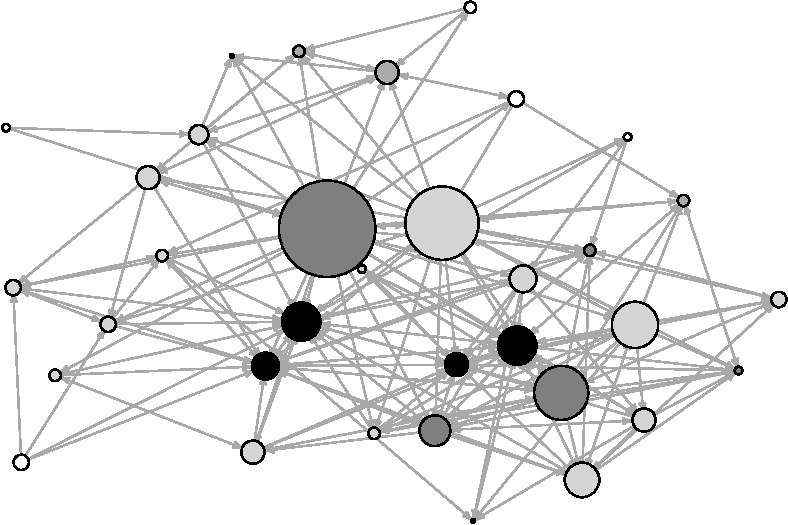
\includegraphics[width=1\textwidth]{dvNet}
	\caption{dv net}
	\label{fig:dvNet}
\end{figure}

\citet{krivitsky:handcock:2015}

\subsection{Parameter Estimates}

% latex table generated in R 3.3.1 by xtable 1.8-2 package
% Sun Aug 21 03:32:43 2016
\begin{table}[ht]
\centering
\begingroup\normalsize
\begin{tabular}{lccccc}
   & Logit & MRQAP & LSM & ERGM & AME \\ 
  \hline
\hline
Intercept/Edges & -4.44$^{\ast}$ & -4.24$^{\ast}$ & 0.94$^{\ast}$ & -12.17$^{\ast}$ & -3.39$^{\ast}$ \\ 
   & (0.34) &  & [0.09; 1.82] & (1.40) & [-4.38; -2.50] \\ 
  \textbf{Conflicting policy preferences} &  &  &  &  &  \\ 
  $\;\;\;\;$ Business vs. NGO & -0.86 & -0.87$^{\ast}$ & -1.37$^{\ast}$ & -1.11$^{\ast}$ & -1.37$^{\ast}$ \\ 
   & (0.46) &  & [-2.42; -0.41] & (0.51) & [-2.44; -0.47] \\ 
  $\;\;\;\;$ Opposition/alliance & 1.21$^{\ast}$ & 1.14$^{\ast}$ & 0.00 & 1.22$^{\ast}$ & 1.08$^{\ast}$ \\ 
   & (0.20) &  & [-0.40; 0.39] & (0.20) & [0.72; 1.47] \\ 
  $\;\;\;\;$ Preference dissimilarity & -0.07 & -0.60 & -1.76$^{\ast}$ & -0.44 & -0.79$^{\ast}$ \\ 
   & (0.37) &  & [-2.62; -0.90] & (0.39) & [-1.55; -0.08] \\ 
  \textbf{Transaction costs} &  &  &  &  &  \\ 
  $\;\;\;\;$ Joint forum participation & 0.88$^{\ast}$ & 0.75$^{\ast}$ & 1.51$^{\ast}$ & 0.90$^{\ast}$ & 0.92$^{\ast}$ \\ 
   & (0.27) &  & [0.86; 2.17] & (0.28) & [0.40; 1.47] \\ 
  \textbf{Influence} &  &  &  &  &  \\ 
  $\;\;\;\;$ Influence attribution & 1.20$^{\ast}$ & 1.29$^{\ast}$ & 0.08 & 1.00$^{\ast}$ & 1.09$^{\ast}$ \\ 
   & (0.22) &  & [-0.40; 0.55] & (0.21) & [0.69; 1.53] \\ 
  $\;\;\;\;$ Alter's influence indegree & 0.10$^{\ast}$ & 0.11$^{\ast}$ & 0.01 & 0.21$^{\ast}$ & 0.11$^{\ast}$ \\ 
   & (0.02) &  & [-0.03; 0.04] & (0.04) & [0.07; 0.15] \\ 
  $\;\;\;\;$ Influence absolute diff. & -0.03$^{\ast}$ & -0.06$^{\ast}$ & 0.04 & -0.05$^{\ast}$ & -0.07$^{\ast}$ \\ 
   & (0.02) &  & [-0.01; 0.09] & (0.01) & [-0.11; -0.03] \\ 
  $\;\;\;\;$ Alter = Government actor & 0.63$^{\ast}$ & 0.68 & -0.46 & 1.04$^{\ast}$ & 0.55 \\ 
   & (0.25) &  & [-1.08; 0.14] & (0.34) & [-0.07; 1.15] \\ 
  \textbf{Functional requirements} &  &  &  &  &  \\ 
  $\;\;\;\;$ Ego = Environmental NGO & 0.88$^{\ast}$ & 0.99 & -0.60 & 0.79$^{\ast}$ & 0.67 \\ 
   & (0.26) &  & [-1.32; 0.09] & (0.17) & [-0.38; 1.71] \\ 
  $\;\;\;\;$ Same actor type & 0.74$^{\ast}$ & 1.12$^{\ast}$ & 1.17$^{\ast}$ & 0.99$^{\ast}$ & 1.04$^{\ast}$ \\ 
   & (0.22) &  & [0.63; 1.71] & (0.23) & [0.63; 1.50] \\ 
  \textbf{Endogenous dependencies} &  &  &  &  &  \\ 
  $\;\;\;\;$ Mutuality & 1.22$^{\ast}$ & 1.00$^{\ast}$ &  & 0.81$^{\ast}$ & 0.39 \\ 
   & (0.21) &  &  & (0.25) & [-0.12; 0.96] \\ 
  $\;\;\;\;$ Outdegree popularity &  &  &  & 0.95$^{\ast}$ &  \\ 
   &  &  &  & (0.09) &  \\ 
  $\;\;\;\;$ Twopaths &  &  &  & -0.04$^{\ast}$ &  \\ 
   &  &  &  & (0.02) &  \\ 
  $\;\;\;\;$ GWIdegree (2.0) &  &  &  & 3.42$^{\ast}$ &  \\ 
   &  &  &  & (1.47) &  \\ 
  $\;\;\;\;$ GWESP (1.0) &  &  &  & 0.58$^{\ast}$ &  \\ 
   &  &  &  & (0.16) &  \\ 
  $\;\;\;\;$ GWOdegree (0.5) &  &  &  & 8.42$^{\ast}$ &  \\ 
   &  &  &  & (2.11) &  \\ 
   \hline
\hline
\end{tabular}
\endgroup
\caption{* p $<$ 0.05. Logistic regression and ERGM results are shown with standard errors in parentheses. MRQAP provides no standard errors. LSM and AME are shown with 95\% posterior credible intervals provided in brackets.} 
\label{tab:regTable}
\end{table}


\subsection{Capturing Network Attributes}

To assess whether the model adequately captures the network parameters of the DV. Here we compare the observed with a set of simulated networks based on certain network statistics \citep{hunter:etal:2008}. 

See \citet{morris:etal:2008} for details on each of these parameters. 

\begin{itemize}
\item Dyad-wise shared partners - Number of dyads in the network with exactly $i$ shared partners
\item Edge-wise shared partners - Similar to above except this counts the number of dyads with the same number of edges
\item Geodesic distances - The proportion of pairs of nodes whose shortest connecting path is of length $k$, for $k=1,2,\ldots$ Also, pairs of nodes that are not connected are classified as $k=\infty$.
\item Incoming k-star - Propensities for individuals to have connections with multiple network partners
\item Indegree - degree count is the number of nodes with the same value of the attribute as the ego node
\item Outdegree - degree count is the number of nodes with the same value of the attribute as the ego node
\end{itemize}

\begin{figure}[ht]
	\centering
	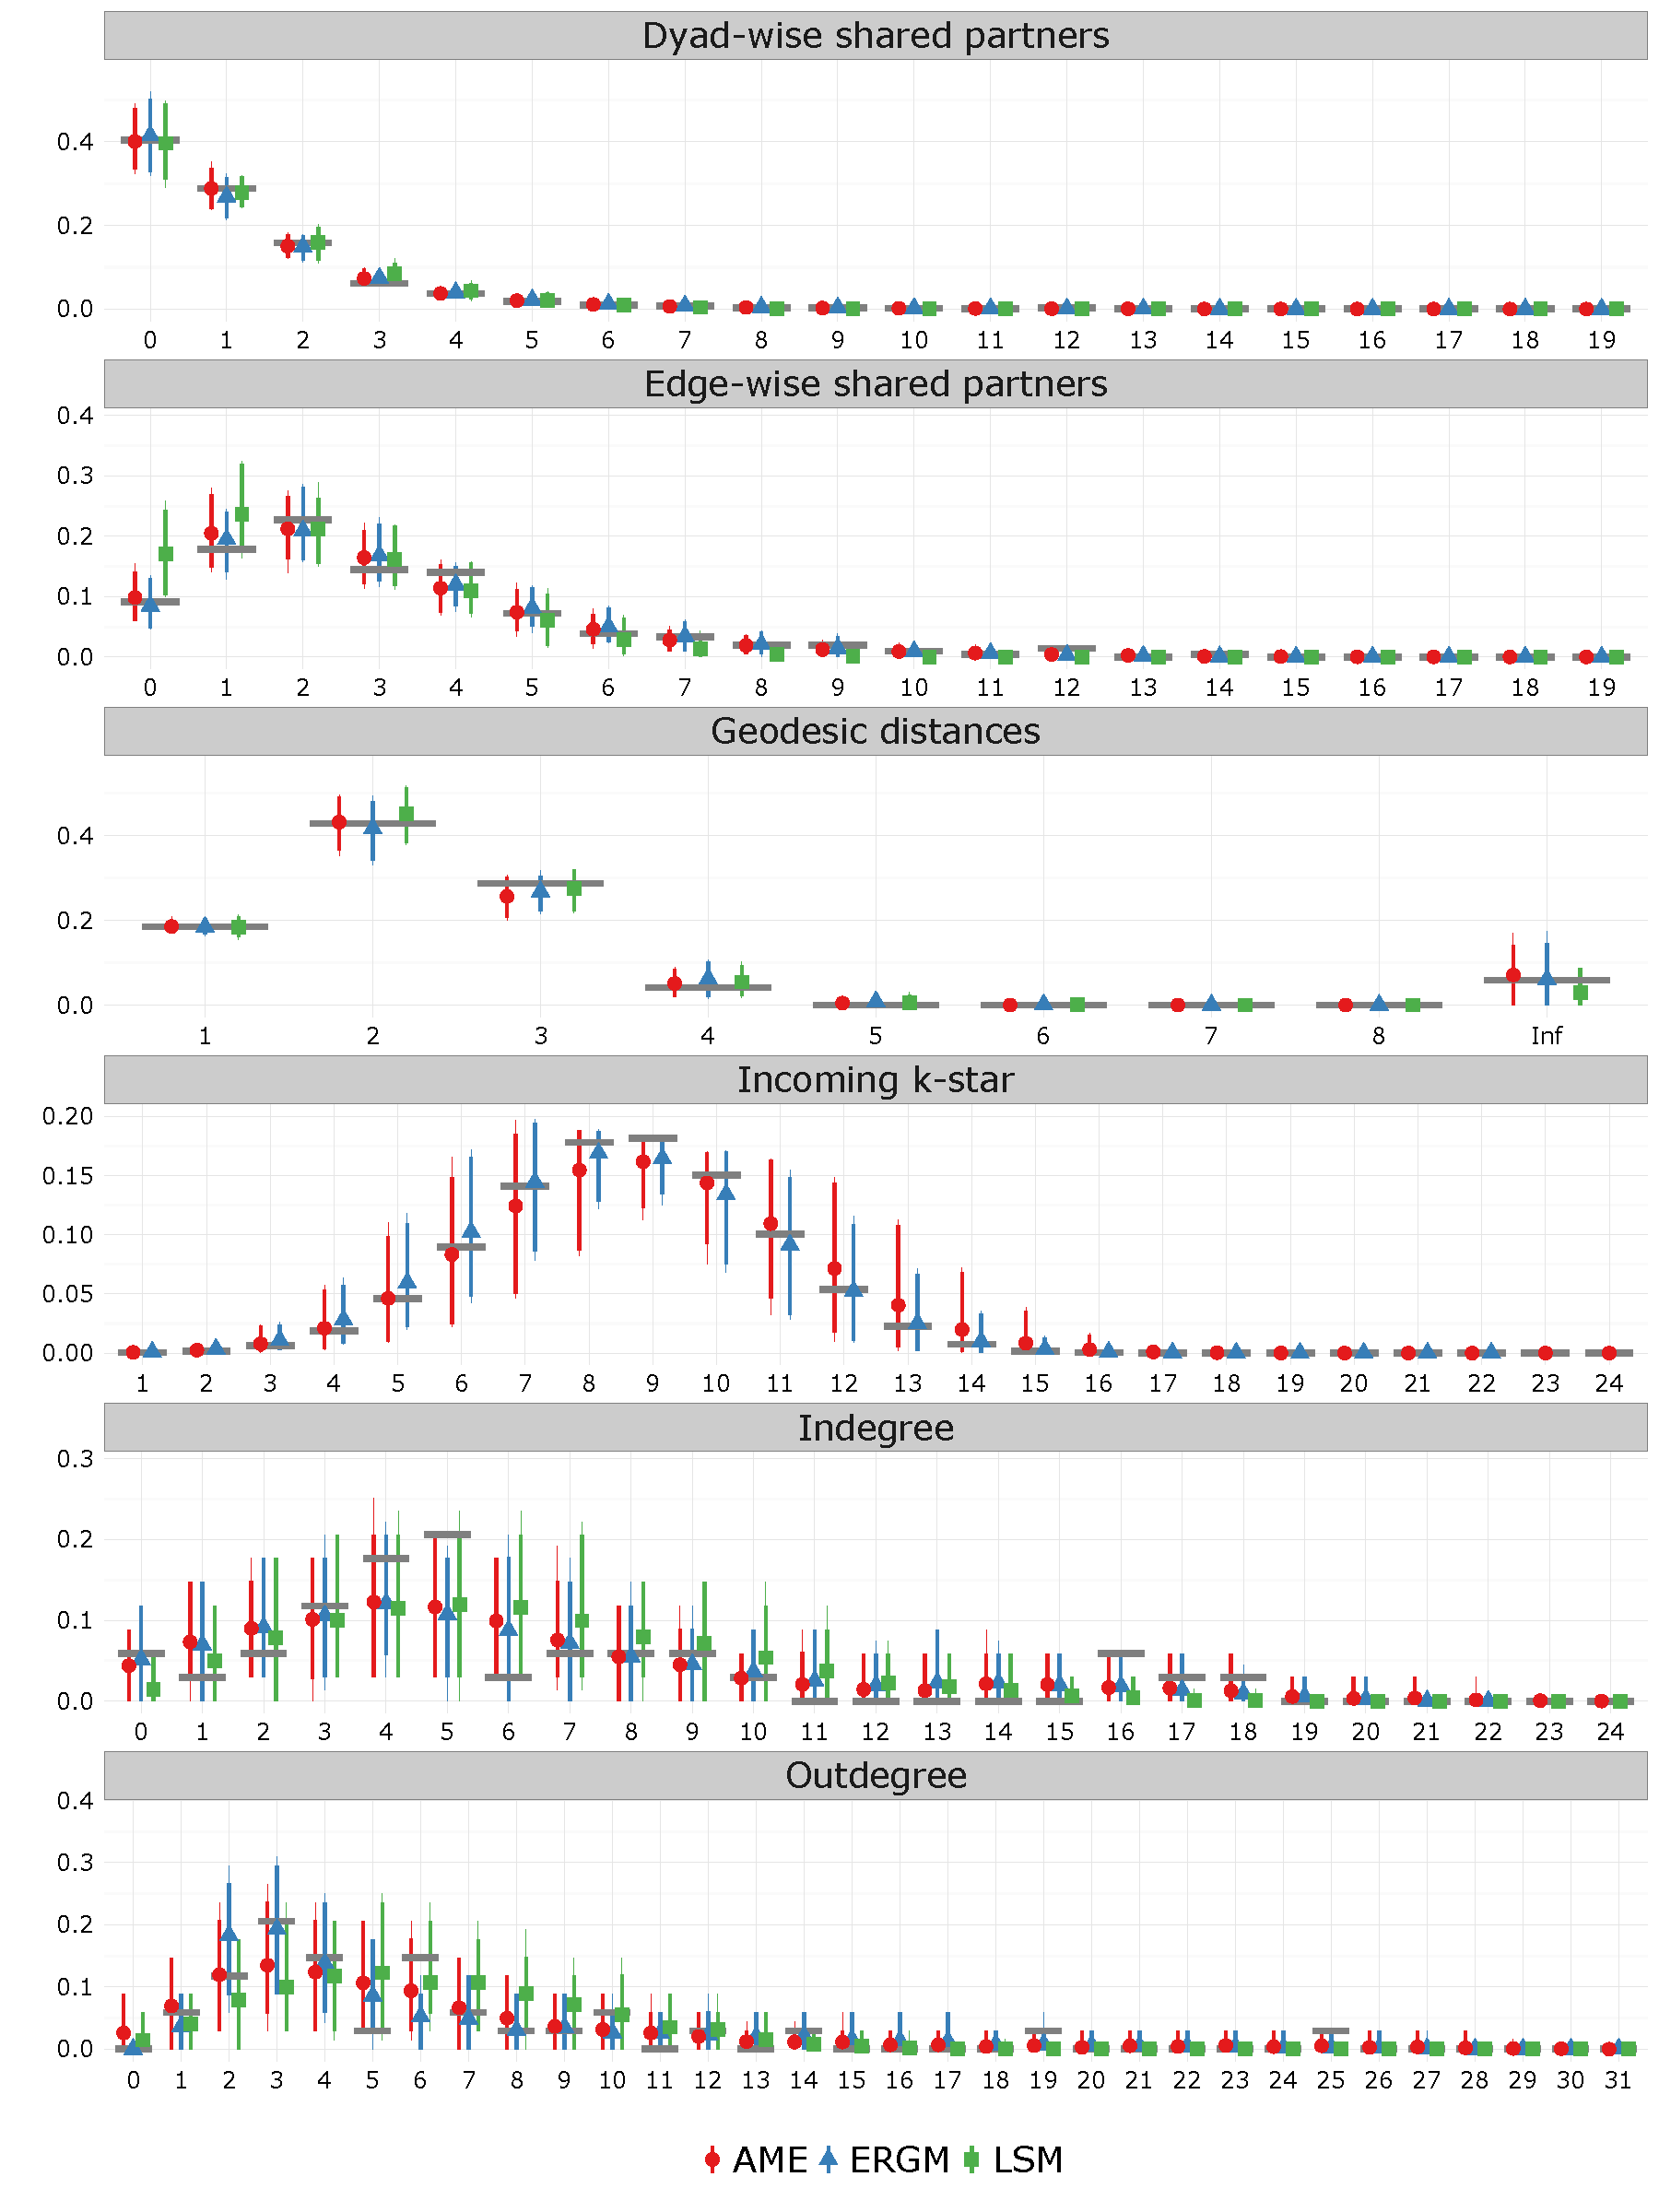
\includegraphics[width=1\textwidth]{ggGofAll}
	\caption{network stats }
	\label{fig:gofAll}
\end{figure}

Figure~\ref{fig:ergmAmePerf} give posterior predictive goodness of fit summaries for four network statistics: (1) the empirical standard deviation of the row means; (2) the empirical standard deviation of the column means (heterogeneity of nodes with incoming activity); (3) the empirical within-dyad correlation; (4) a normalized measure of triadic dependence \citep{hoff:etal:2015}. 

For a given summary statistic g() we first simulate $\mathbf{Y}_{sim} \approx p(\mathbf{Y}_{sim} | \mathbf{Y}_{obs}) = \int p(\mathbf{Y}_{sim} | \theta) p(d \theta | \mathbf{Y}_{obs})$ and then we compare $g(\mathbf{Y}_{sim})$ to $g(\mathbf{Y}_{obs})$. Histograms represent predicted value of statistics under the model and red dash line represents the observed value. 

Proportion of ties that are reciprocated. 

\begin{align}
\begin{aligned}
t(Y) &= \frac{ \sum_{i \neq j}y_{i,j} y_{j,i} }{ \sum_{i \neq j} y_{i,j} } \\
\end{aligned}
\end{align}

Number of transitive triplets, number of triangles in network, number of times ijk are all connected.

\begin{align}
\begin{aligned}
t(Y) &= \sum_{i \neq j \neq k} y_{i,j} y_{i,k} y_{j,k}
\end{aligned}
\end{align}

\begin{figure}[ht]
	\centering
	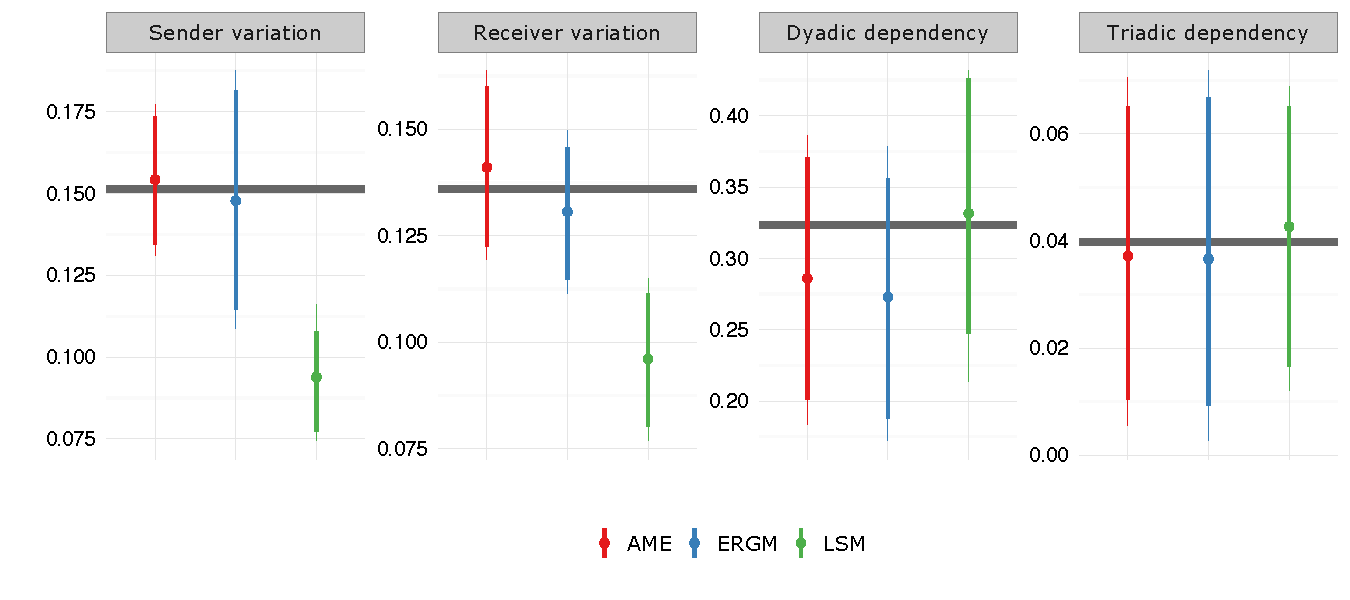
\includegraphics[width=1\textwidth]{netPerfCoef}
	\caption{Posterior predictive goodness of fit summary}
	\label{fig:ergmAmePerf}
\end{figure}

\subsection{Tie Formation Prediction}

The results are displayed in Figure \ref{fig:roc} using separation plots and Receiver Operating Characteristic (ROC) curves.

We compare the sensitivity and specificity trade-off for each model using ROC curves. Models that have a better fit according to this test should have curves that follow the left-hand border and then the top border of the ROC space. Here again it is apparent that accounting for the interstate relations and the endogenous network effects leads to noticeable improvements in performance. Last, by calculating the area under the ROC curve (AUC) we can assess the accuracy of each model.

Separation plots provide a visual interpretation of model fit by plotting all observations, in this case country pairs, in the data set according to their predicted value from left (low values) to right (high values). Models with a good fit should should have all actual (dark blue) observations towards the right of the separation plot \citep{greenhill:etal:2011}.

\citet{beger:2015}

In addition, we also highlight the difference in performance through the utilization of a precision-recall curve. Precision is a measure of result relevancy, while recall is a measure of how many truly relevant results are returned. A high area under the curve represents both high recall and high precision, where high precision relates to a low false positive rate, and high recall relates to a low false negative rate. High scores for both show that the classifier is returning accurate results (high precision), as well as returning a majority of all positive results (high recall). 

Precision is defined as the number of true positives over the number of true positives plus the number of false positives. 

Recall is defined as the number of true positives over the number of true positives plus the number of false negatives. 

\begin{figure}[ht]
	\centering
	\begin{tabular}{cc}
	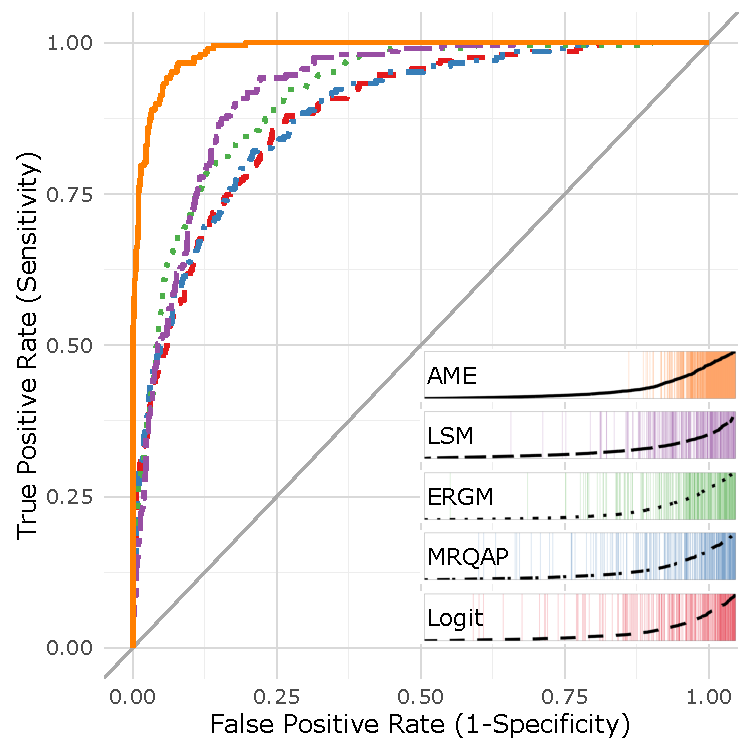
\includegraphics[width=.5\textwidth]{roc} & 
	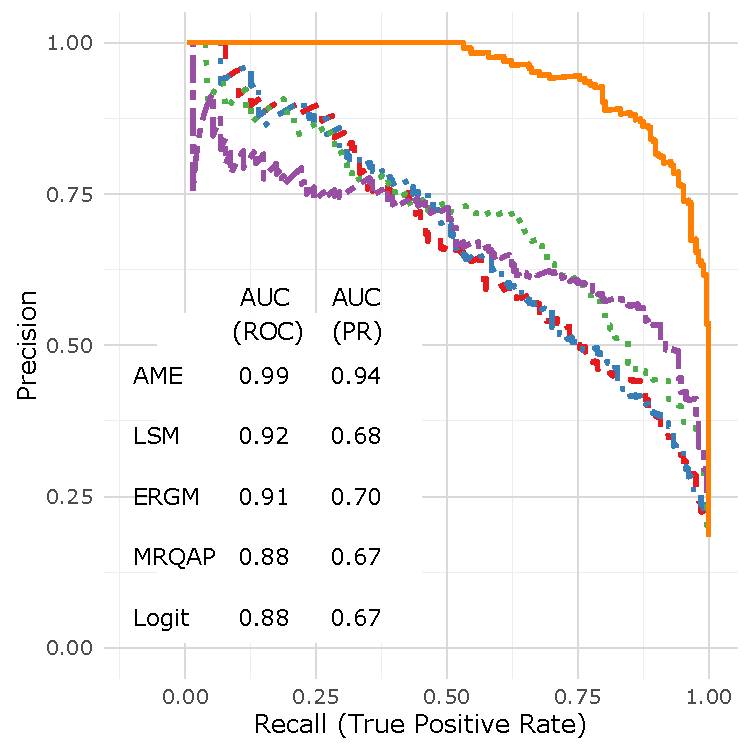
\includegraphics[width=.5\textwidth]{rocPr}	
	\end{tabular}
	\caption{ROC and separation plots}
	\label{fig:roc}
\end{figure}

% % latex table generated in R 3.3.1 by xtable 1.8-2 package
% Tue Oct 18 00:16:48 2016
\begin{table}[ht]
\centering
\begingroup\normalsize
\begin{tabular}{lcc}
  & AUC & AUC (PR) \\ 
  \hline
\hline
AME & 0.99 & 0.94 \\ 
  LSM & 0.92 & 0.68 \\ 
  ERGM & 0.91 & 0.70 \\ 
  MRQAP & 0.88 & 0.67 \\ 
  Logit & 0.88 & 0.67 \\ 
  \end{tabular}
\endgroup
\caption{Area under the curve (AUC) comparison.} 
\label{tab:aucTable}
\end{table}

\section{Conclusion}



\newpage
\section{Appendix}

\section{AMEN Model Convergence}

\begin{figure}[ht]
	\centering
	\begin{tabular}{cc}
	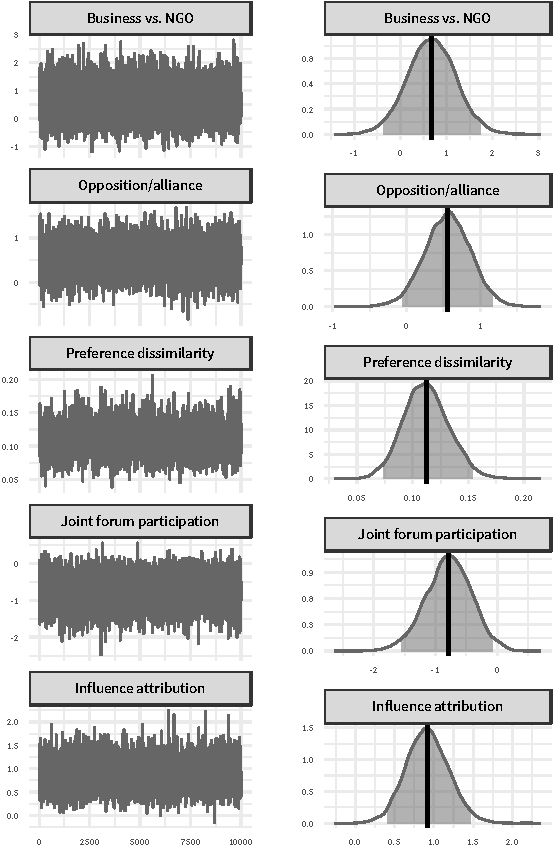
\includegraphics[width=.45\textwidth]{ameConv1_SR2} &
	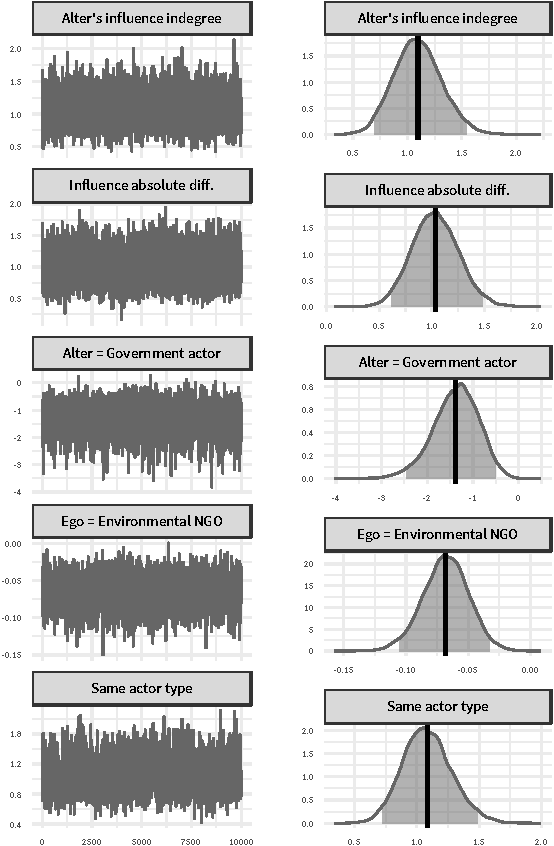
\includegraphics[width=.45\textwidth]{ameConv2_SR2}
	\end{tabular}
	\caption{ame convergence k = 2}
	\label{fig:ameConv}
\end{figure}
\FloatBarrier
\newpage

\section{Comparison of \pkg{amen} \& \pkg{latentnet} $\mathcal{R}$ Packages}

% latex table generated in R 3.3.1 by xtable 1.8-2 package
% Sun Aug 21 03:38:39 2016
\begin{table}[ht]
\centering
\begingroup\tiny
\begin{tabular}{lccccc}
   & LSM & LSM (Bilinear) & LSM (SR) & LSM (Bilinear + SR) & AME \\ 
  \hline
\hline
Intercept/Edges & 0.94$^{\ast}$ & -2.66$^{\ast}$ & 0.60 & -2.50$^{\ast}$ & -3.39$^{\ast}$ \\ 
   & [0.09; 1.82] & [-3.53; -1.87] & [-1.10; 2.37] & [-4.14; -0.88] & [-4.38; -2.50] \\ 
  \textbf{Conflicting policy preferences} &  &  &  &  &  \\ 
  $\;\;\;\;$ Business vs. NGO & -1.37$^{\ast}$ & -2.64$^{\ast}$ & -3.07$^{\ast}$ & -2.87$^{\ast}$ & -1.37$^{\ast}$ \\ 
   & [-2.42; -0.41] & [-4.61; -0.96] & [-4.77; -1.56] & [-4.63; -1.29] & [-2.44; -0.47] \\ 
  $\;\;\;\;$ Opposition/alliance & 0.00 & 0.04 & 0.31 & 0.24 & 1.08$^{\ast}$ \\ 
   & [-0.40; 0.39] & [-0.44; 0.54] & [-0.24; 0.86] & [-0.36; 0.82] & [0.72; 1.47] \\ 
  $\;\;\;\;$ Preference dissimilarity & -1.76$^{\ast}$ & -2.00$^{\ast}$ & -1.88$^{\ast}$ & -2.20$^{\ast}$ & -0.79$^{\ast}$ \\ 
   & [-2.62; -0.90] & [-3.01; -1.03] & [-3.07; -0.68] & [-3.46; -0.96] & [-1.55; -0.08] \\ 
  \textbf{Transaction costs} &  &  &  &  &  \\ 
  $\;\;\;\;$ Joint forum participation & 1.51$^{\ast}$ & 1.24$^{\ast}$ & 1.56$^{\ast}$ & 1.62$^{\ast}$ & 0.92$^{\ast}$ \\ 
   & [0.86; 2.17] & [0.53; 1.93] & [0.69; 2.41] & [0.70; 2.52] & [0.40; 1.47] \\ 
  \textbf{Influence} &  &  &  &  &  \\ 
  $\;\;\;\;$ Influence attribution & 0.08 & -0.08 & 0.30 & 0.28 & 1.09$^{\ast}$ \\ 
   & [-0.40; 0.55] & [-0.62; 0.46] & [-0.37; 0.96] & [-0.42; 0.97] & [0.69; 1.53] \\ 
  $\;\;\;\;$ Alter's influence indegree & 0.01 & -0.05$^{\ast}$ & 0.06 & 0.05 & 0.11$^{\ast}$ \\ 
   & [-0.03; 0.04] & [-0.09; -0.01] & [-0.03; 0.14] & [-0.04; 0.13] & [0.07; 0.15] \\ 
  $\;\;\;\;$ Influence absolute diff. & 0.04 & 0.02 & -0.08$^{\ast}$ & -0.08$^{\ast}$ & -0.07$^{\ast}$ \\ 
   & [-0.01; 0.09] & [-0.03; 0.07] & [-0.14; -0.02] & [-0.14; -0.02] & [-0.11; -0.03] \\ 
  $\;\;\;\;$ Alter = Government actor & -0.46 & -0.80 & -0.11 & -0.20 & 0.55 \\ 
   & [-1.08; 0.14] & [-1.67; 0.04] & [-1.91; 1.76] & [-2.14; 1.74] & [-0.07; 1.15] \\ 
  \textbf{Functional requirements} &  &  &  &  &  \\ 
  $\;\;\;\;$ Ego = Environmental NGO & -0.60 & -1.90$^{\ast}$ & -1.69 & -1.84 & 0.67 \\ 
   & [-1.32; 0.09] & [-3.10; -0.86] & [-3.74; 0.23] & [-4.02; 0.11] & [-0.38; 1.71] \\ 
  $\;\;\;\;$ Same actor type & 1.17$^{\ast}$ & 1.40$^{\ast}$ & 1.82$^{\ast}$ & 1.90$^{\ast}$ & 1.04$^{\ast}$ \\ 
   & [0.63; 1.71] & [0.85; 1.95] & [1.10; 2.54] & [1.19; 2.62] & [0.63; 1.50] \\ 
   \hline
\hline
\end{tabular}
\endgroup
\caption{* p $<$ 0.05. 95\% posterior credible intervals are provided in brackets.} 
\label{tab:regTable_latSpace}
\end{table}


% % latex table generated in R 3.3.1 by xtable 1.8-2 package
% Tue Oct 18 00:16:32 2016
\begin{table}[ht]
\centering
\begingroup\normalsize
\begin{tabular}{lcc}
  & AUC & AUC (PR) \\ 
  \hline
\hline
AME & 0.99 & 0.94 \\ 
  LSM (Bilinear + SR) & 0.97 & 0.91 \\ 
  LSM (SR) & 0.97 & 0.90 \\ 
  LSM (Bilinear) & 0.93 & 0.77 \\ 
  LSM & 0.92 & 0.68 \\ 
  \end{tabular}
\endgroup
\caption{Area under the curve (AUC) comparison for latent space approaches.} 
\label{tab:aucTable_latSpace}
\end{table}


\begin{figure}[ht]
	\centering
	\begin{tabular}{cc}
	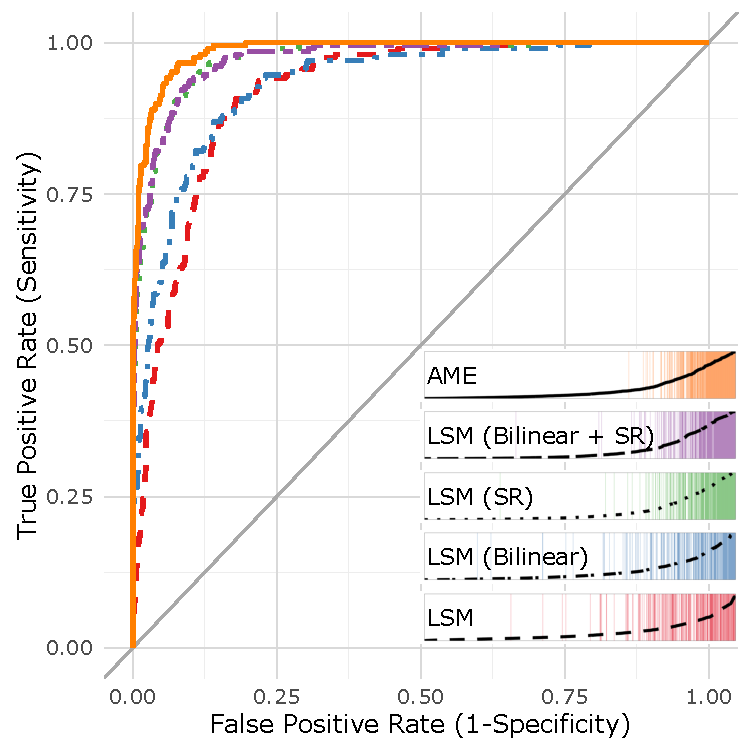
\includegraphics[width=.5\textwidth]{roc_latSpace} & 
	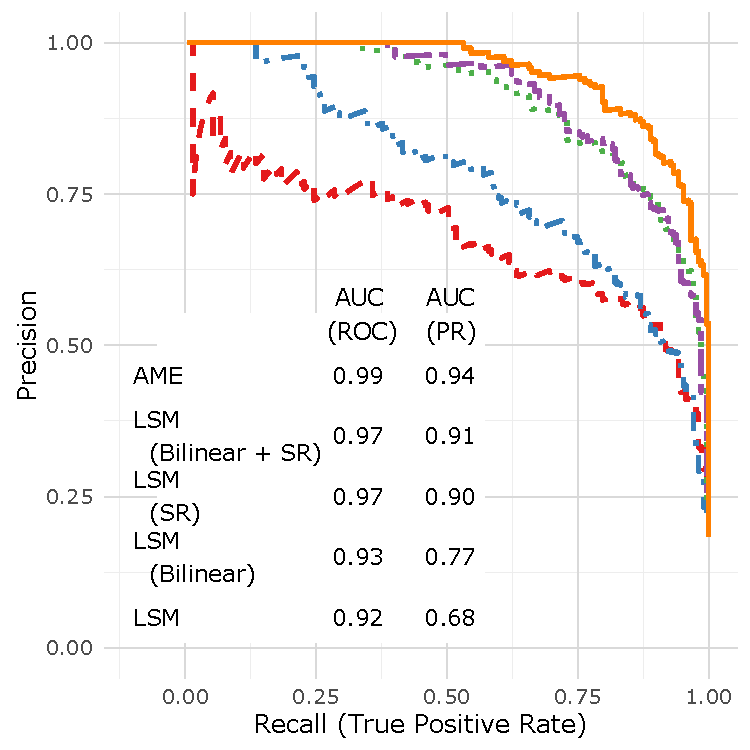
\includegraphics[width=.5\textwidth]{rocPr_latSpace}
	\end{tabular}
	\caption{ROC and separation plots}
	\label{fig:roc_latentSpace}
\end{figure}

\begin{figure}[ht]
	\centering
	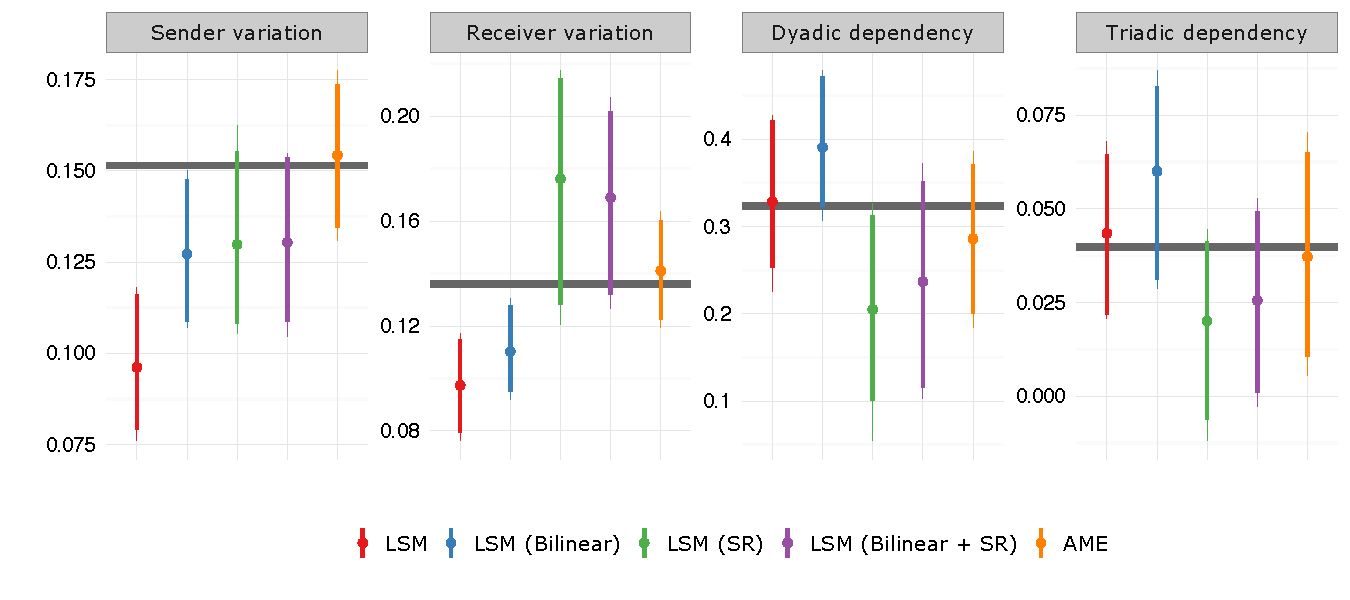
\includegraphics[width=1\textwidth]{netPerfCoef_latSpace}
	\caption{Posterior predictive goodness of fit summary}
	\label{fig:netPerfCoef_latSpace}
\end{figure}

\begin{figure}[ht]
	\centering
	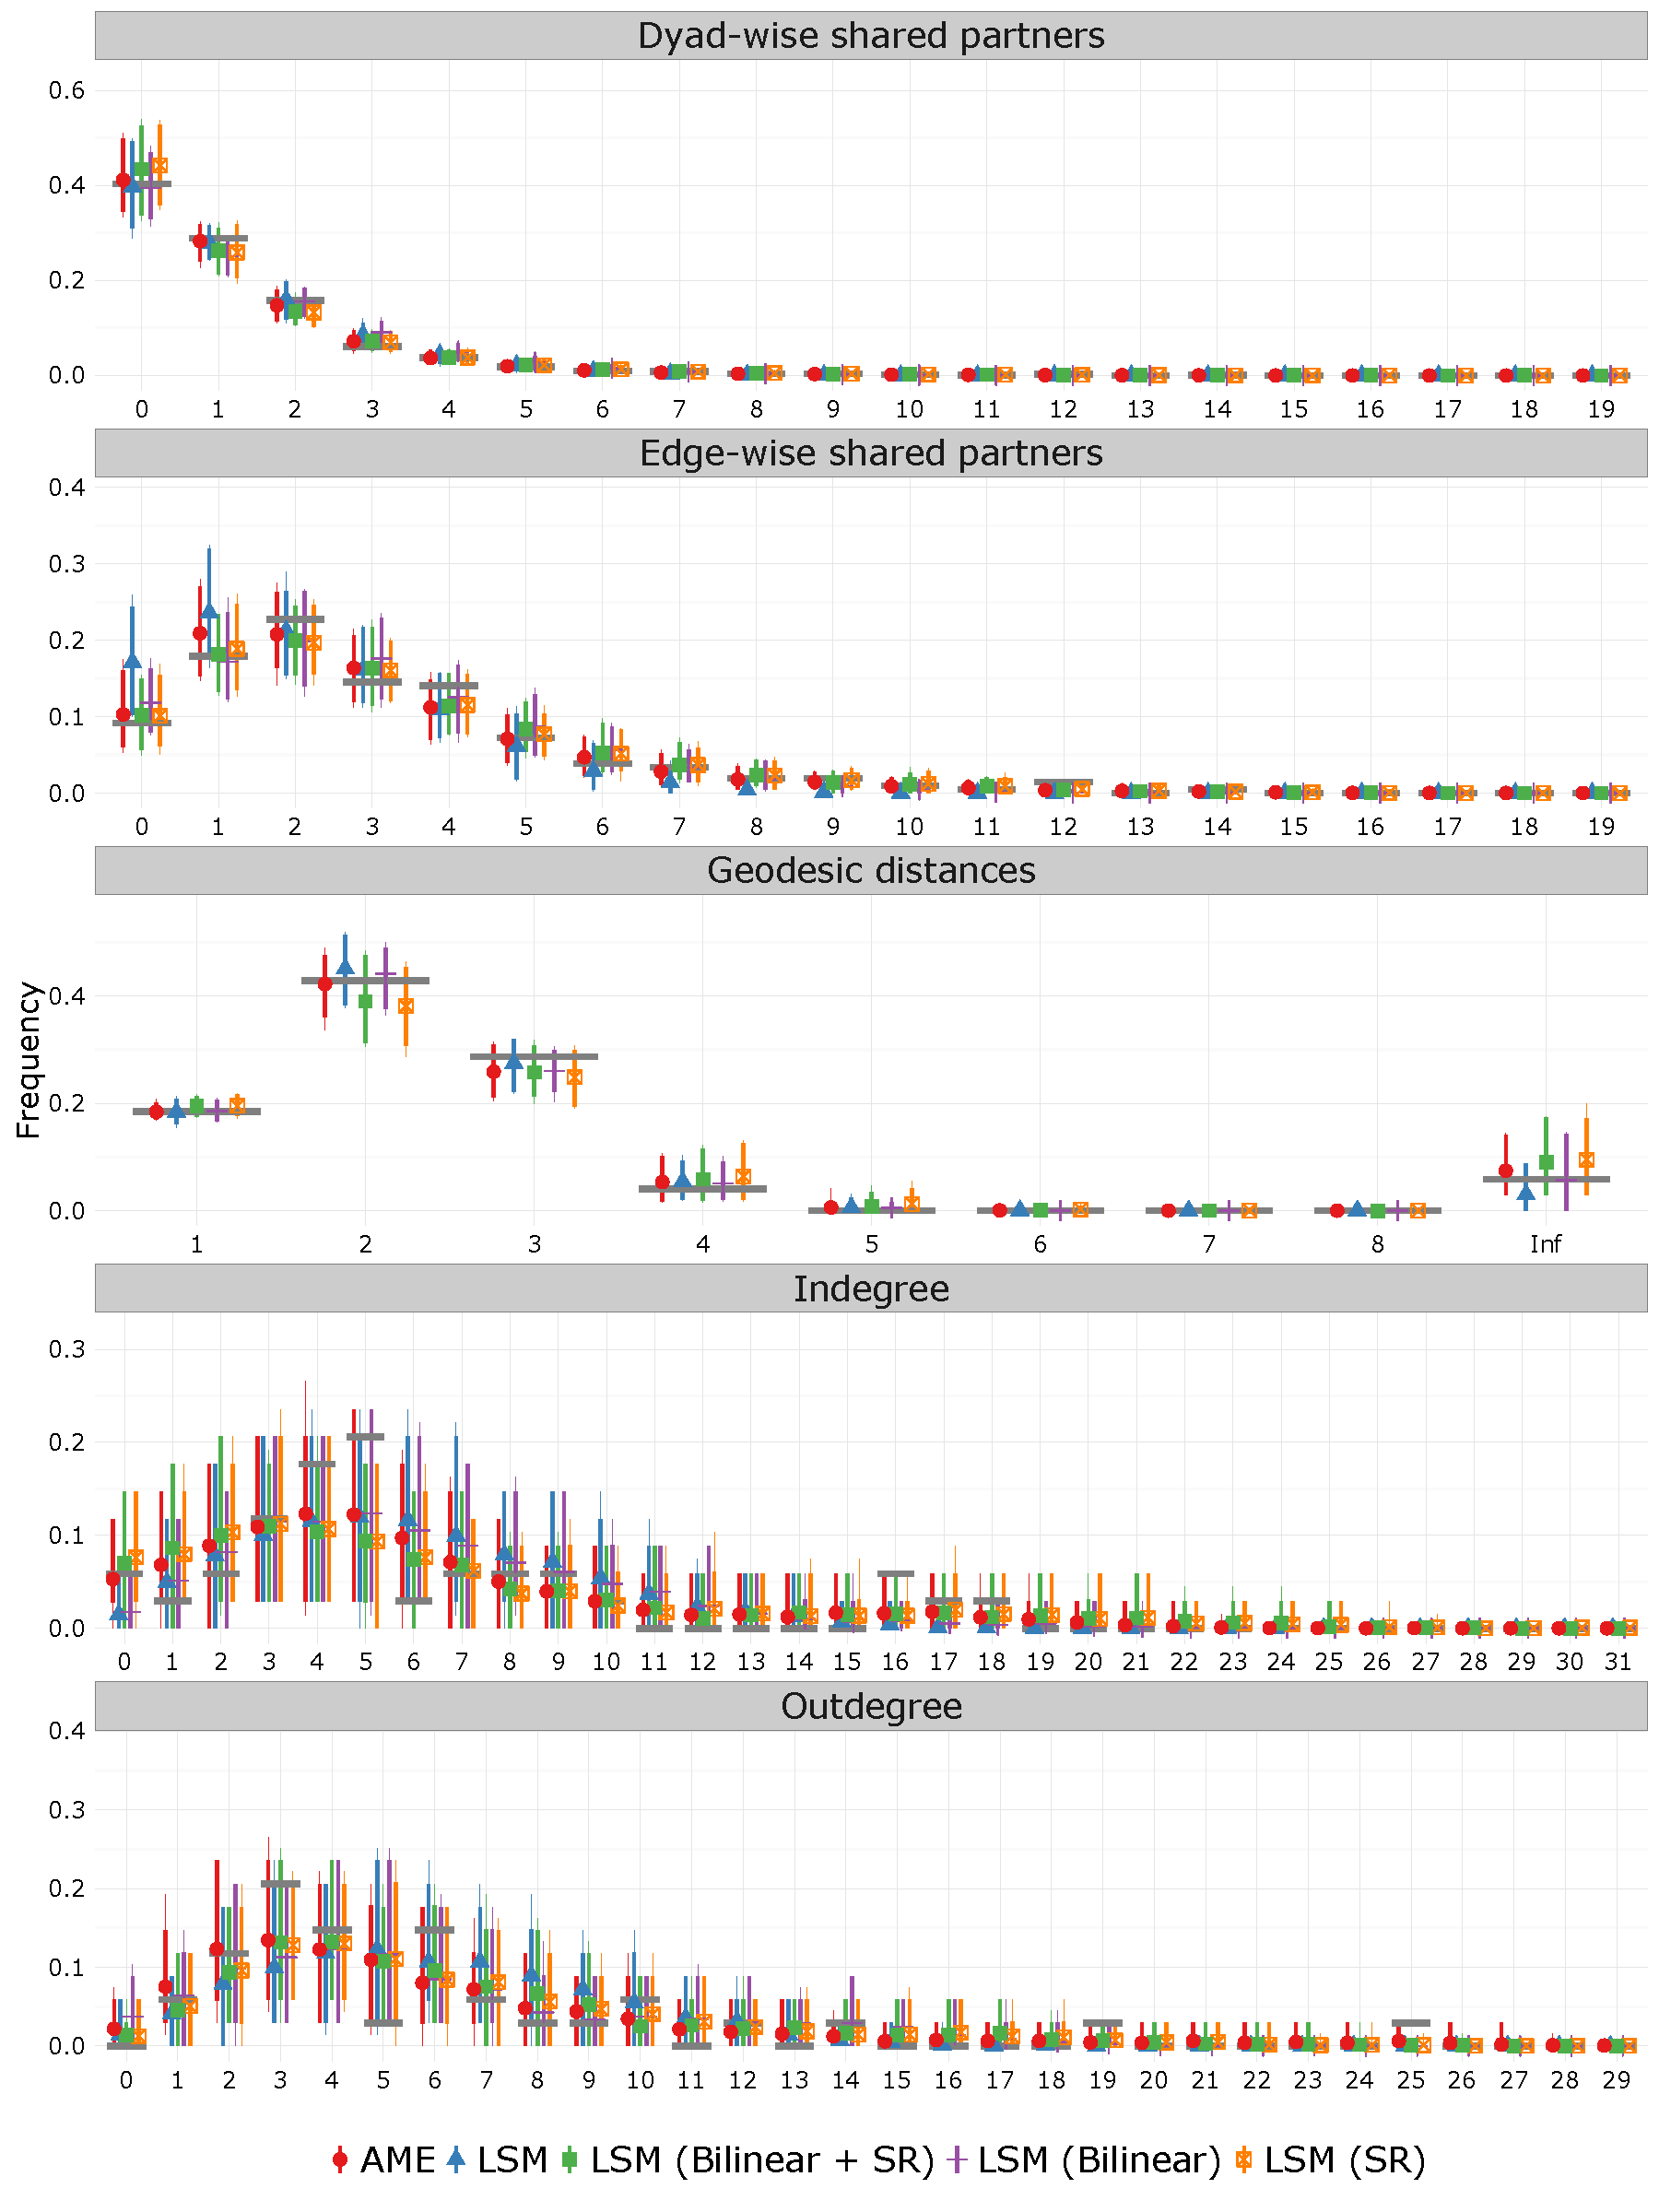
\includegraphics[width=1\textwidth]{ggGofAll_latSpace}
	\caption{network stats }
	\label{fig:gofAll_latSpace}
\end{figure}
\FloatBarrier
\newpage

\section{Comparison with other AME Parameterizations}

% latex table generated in R 3.5.0 by xtable 1.8-2 package
% Wed Jul 11 18:23:00 2018
\begin{table}[ht]
\centering
\begingroup\tiny
\begin{tabular}{lcccc}
   & AME (k=1) & AME (k=2) & AME (k=3) & AME (k=4) \\ 
  \hline
\hline
Intercept/Edges & -3.07 & -3.40 & -3.91 & -4.13 \\ 
   & [-3.87; -2.29] & [-4.40; -2.51] & [-5.90; -2.82] & [-5.93; -3.00] \\ 
  \textbf{Conflicting policy preferences} &  &  &  &  \\ 
  $\;\;\;\;$ Business vs. NGO & -1.27 & -1.38 & -1.52 & -1.54 \\ 
   & [-2.19; -0.47] & [-2.47; -0.49] & [-2.67; -0.53] & [-2.59; -0.47] \\ 
  $\;\;\;\;$ Opposition/alliance & 0.94 & 1.08 & 1.27 & 1.38 \\ 
   & [0.66; 1.27] & [0.72; 1.49] & [0.82; 2.10] & [0.87; 2.24] \\ 
  $\;\;\;\;$ Preference dissimilarity & -0.65 & -0.79 & -0.90 & -0.94 \\ 
   & [-1.28; -0.04] & [-1.55; -0.07] & [-1.78; -0.13] & [-1.77; -0.08] \\ 
  \textbf{Transaction costs} &  &  &  &  \\ 
  $\;\;\;\;$ Joint forum participation & 0.84 & 0.92 & 1.08 & 1.22 \\ 
   & [0.38; 1.31] & [0.40; 1.46] & [0.41; 1.96] & [0.50; 2.24] \\ 
  \textbf{Influence} &  &  &  &  \\ 
  $\;\;\;\;$ Influence attribution & 1.00 & 1.10 & 1.30 & 1.39 \\ 
   & [0.65; 1.40] & [0.70; 1.55] & [0.76; 2.29] & [0.82; 2.27] \\ 
  $\;\;\;\;$ Alter's influence indegree & 0.10 & 0.11 & 0.13 & 0.14 \\ 
   & [0.07; 0.13] & [0.07; 0.15] & [0.09; 0.20] & [0.09; 0.21] \\ 
  $\;\;\;\;$ Influence absolute diff. & -0.06 & -0.07 & -0.08 & -0.09 \\ 
   & [-0.09; -0.03] & [-0.11; -0.03] & [-0.15; -0.04] & [-0.16; -0.04] \\ 
  $\;\;\;\;$ Alter = Government actor & 0.52 & 0.56 & 0.65 & 0.72 \\ 
   & [0.00; 1.08] & [-0.06; 1.16] & [-0.05; 1.49] & [-0.01; 1.48] \\ 
  \textbf{Functional requirements} &  &  &  &  \\ 
  $\;\;\;\;$ Ego = Environmental NGO & 0.62 & 0.68 & 0.84 & 0.86 \\ 
   & [-0.28; 1.53] & [-0.36; 1.73] & [-0.43; 2.40] & [-0.49; 2.32] \\ 
  $\;\;\;\;$ Same actor type & 0.98 & 1.03 & 1.17 & 1.23 \\ 
   & [0.60; 1.37] & [0.62; 1.48] & [0.69; 1.83] & [0.70; 1.96] \\ 
   \hline
\hline
\end{tabular}
\endgroup
\caption{* p $<$ 0.05 (or 0 outside the 95\% confidence interval).} 
\label{tab:regTable_latSpace}
\end{table}


% % latex table generated in R 3.3.1 by xtable 1.8-2 package
% Tue Oct 18 00:16:17 2016
\begin{table}[ht]
\centering
\begingroup\normalsize
\begin{tabular}{lcc}
  & AUC & AUC (PR) \\ 
  \hline
\hline
AME (k=4) & 1.00 & 0.98 \\ 
  AME (k=3) & 0.99 & 0.97 \\ 
  AME (k=2) & 0.99 & 0.94 \\ 
  AME (k=1) & 0.97 & 0.90 \\ 
  \end{tabular}
\endgroup
\caption{Area under the curve (AUC) comparison for latent space approaches.} 
\label{tab:aucTable_latSpace}
\end{table}


\begin{figure}[ht]
	\centering
	\begin{tabular}{cc}
	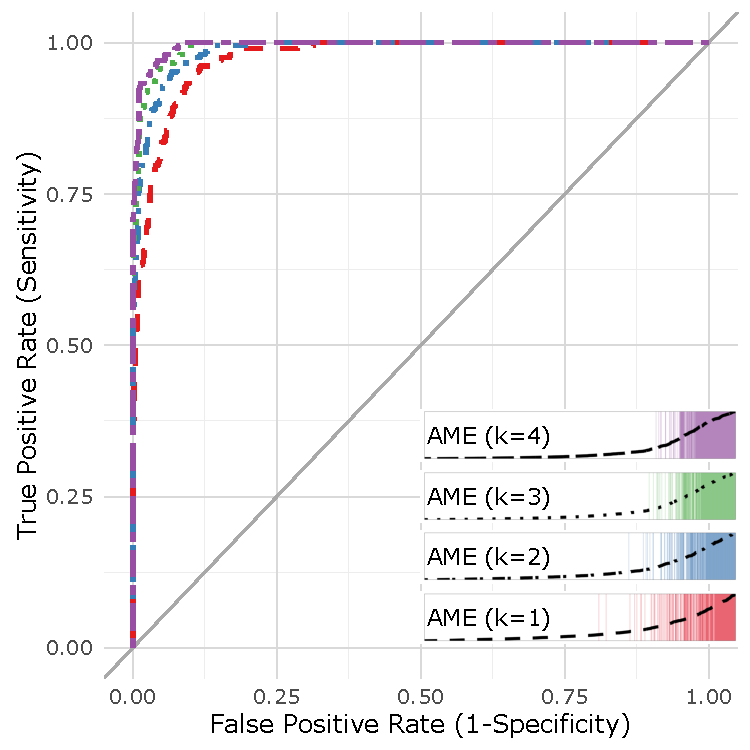
\includegraphics[width=.5\textwidth]{roc_ameSR} & 
	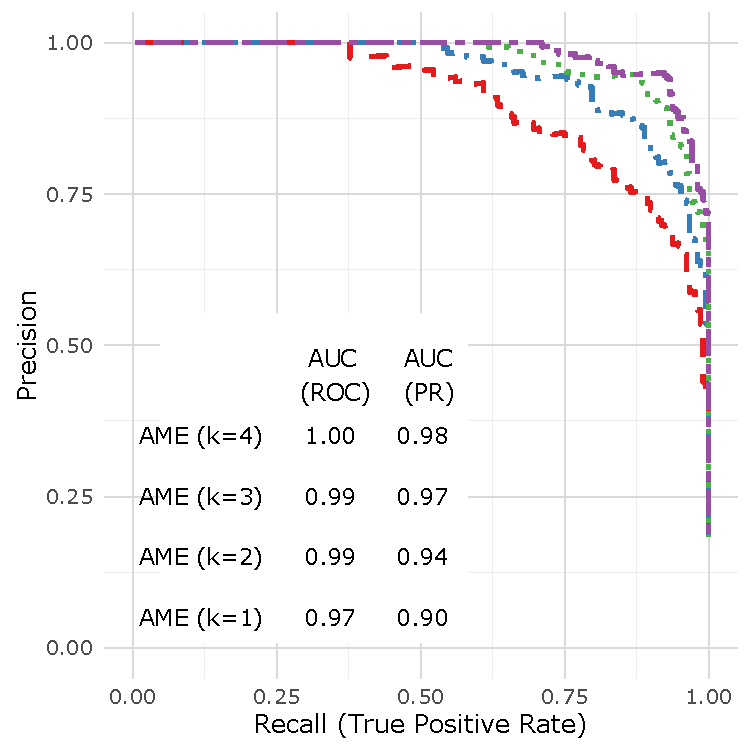
\includegraphics[width=.5\textwidth]{rocPr_ameSR}
	\end{tabular}
	\caption{ROC and separation plots}
	\label{fig:roc_latentSpace}
\end{figure}

\begin{figure}[ht]
	\centering
	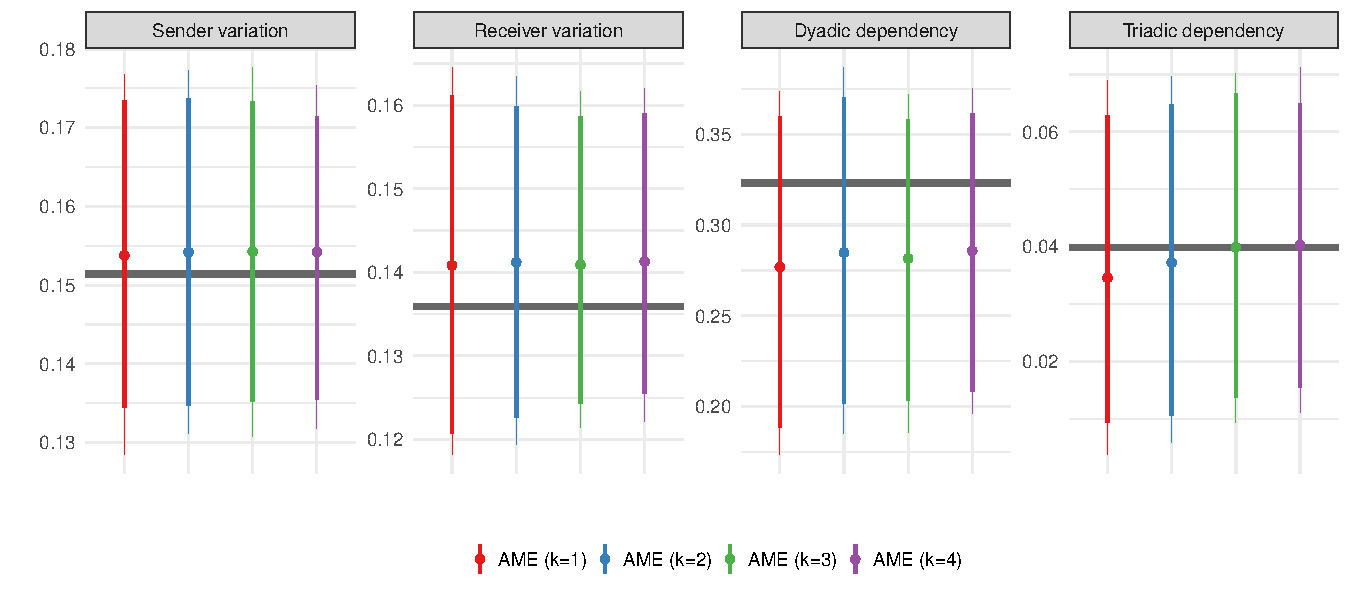
\includegraphics[width=1\textwidth]{netPerfCoef_ameSR}
	\caption{Posterior predictive goodness of fit summary}
	\label{fig:netPerfCoef_ameSR}
\end{figure}

\begin{figure}[ht]
	\centering
	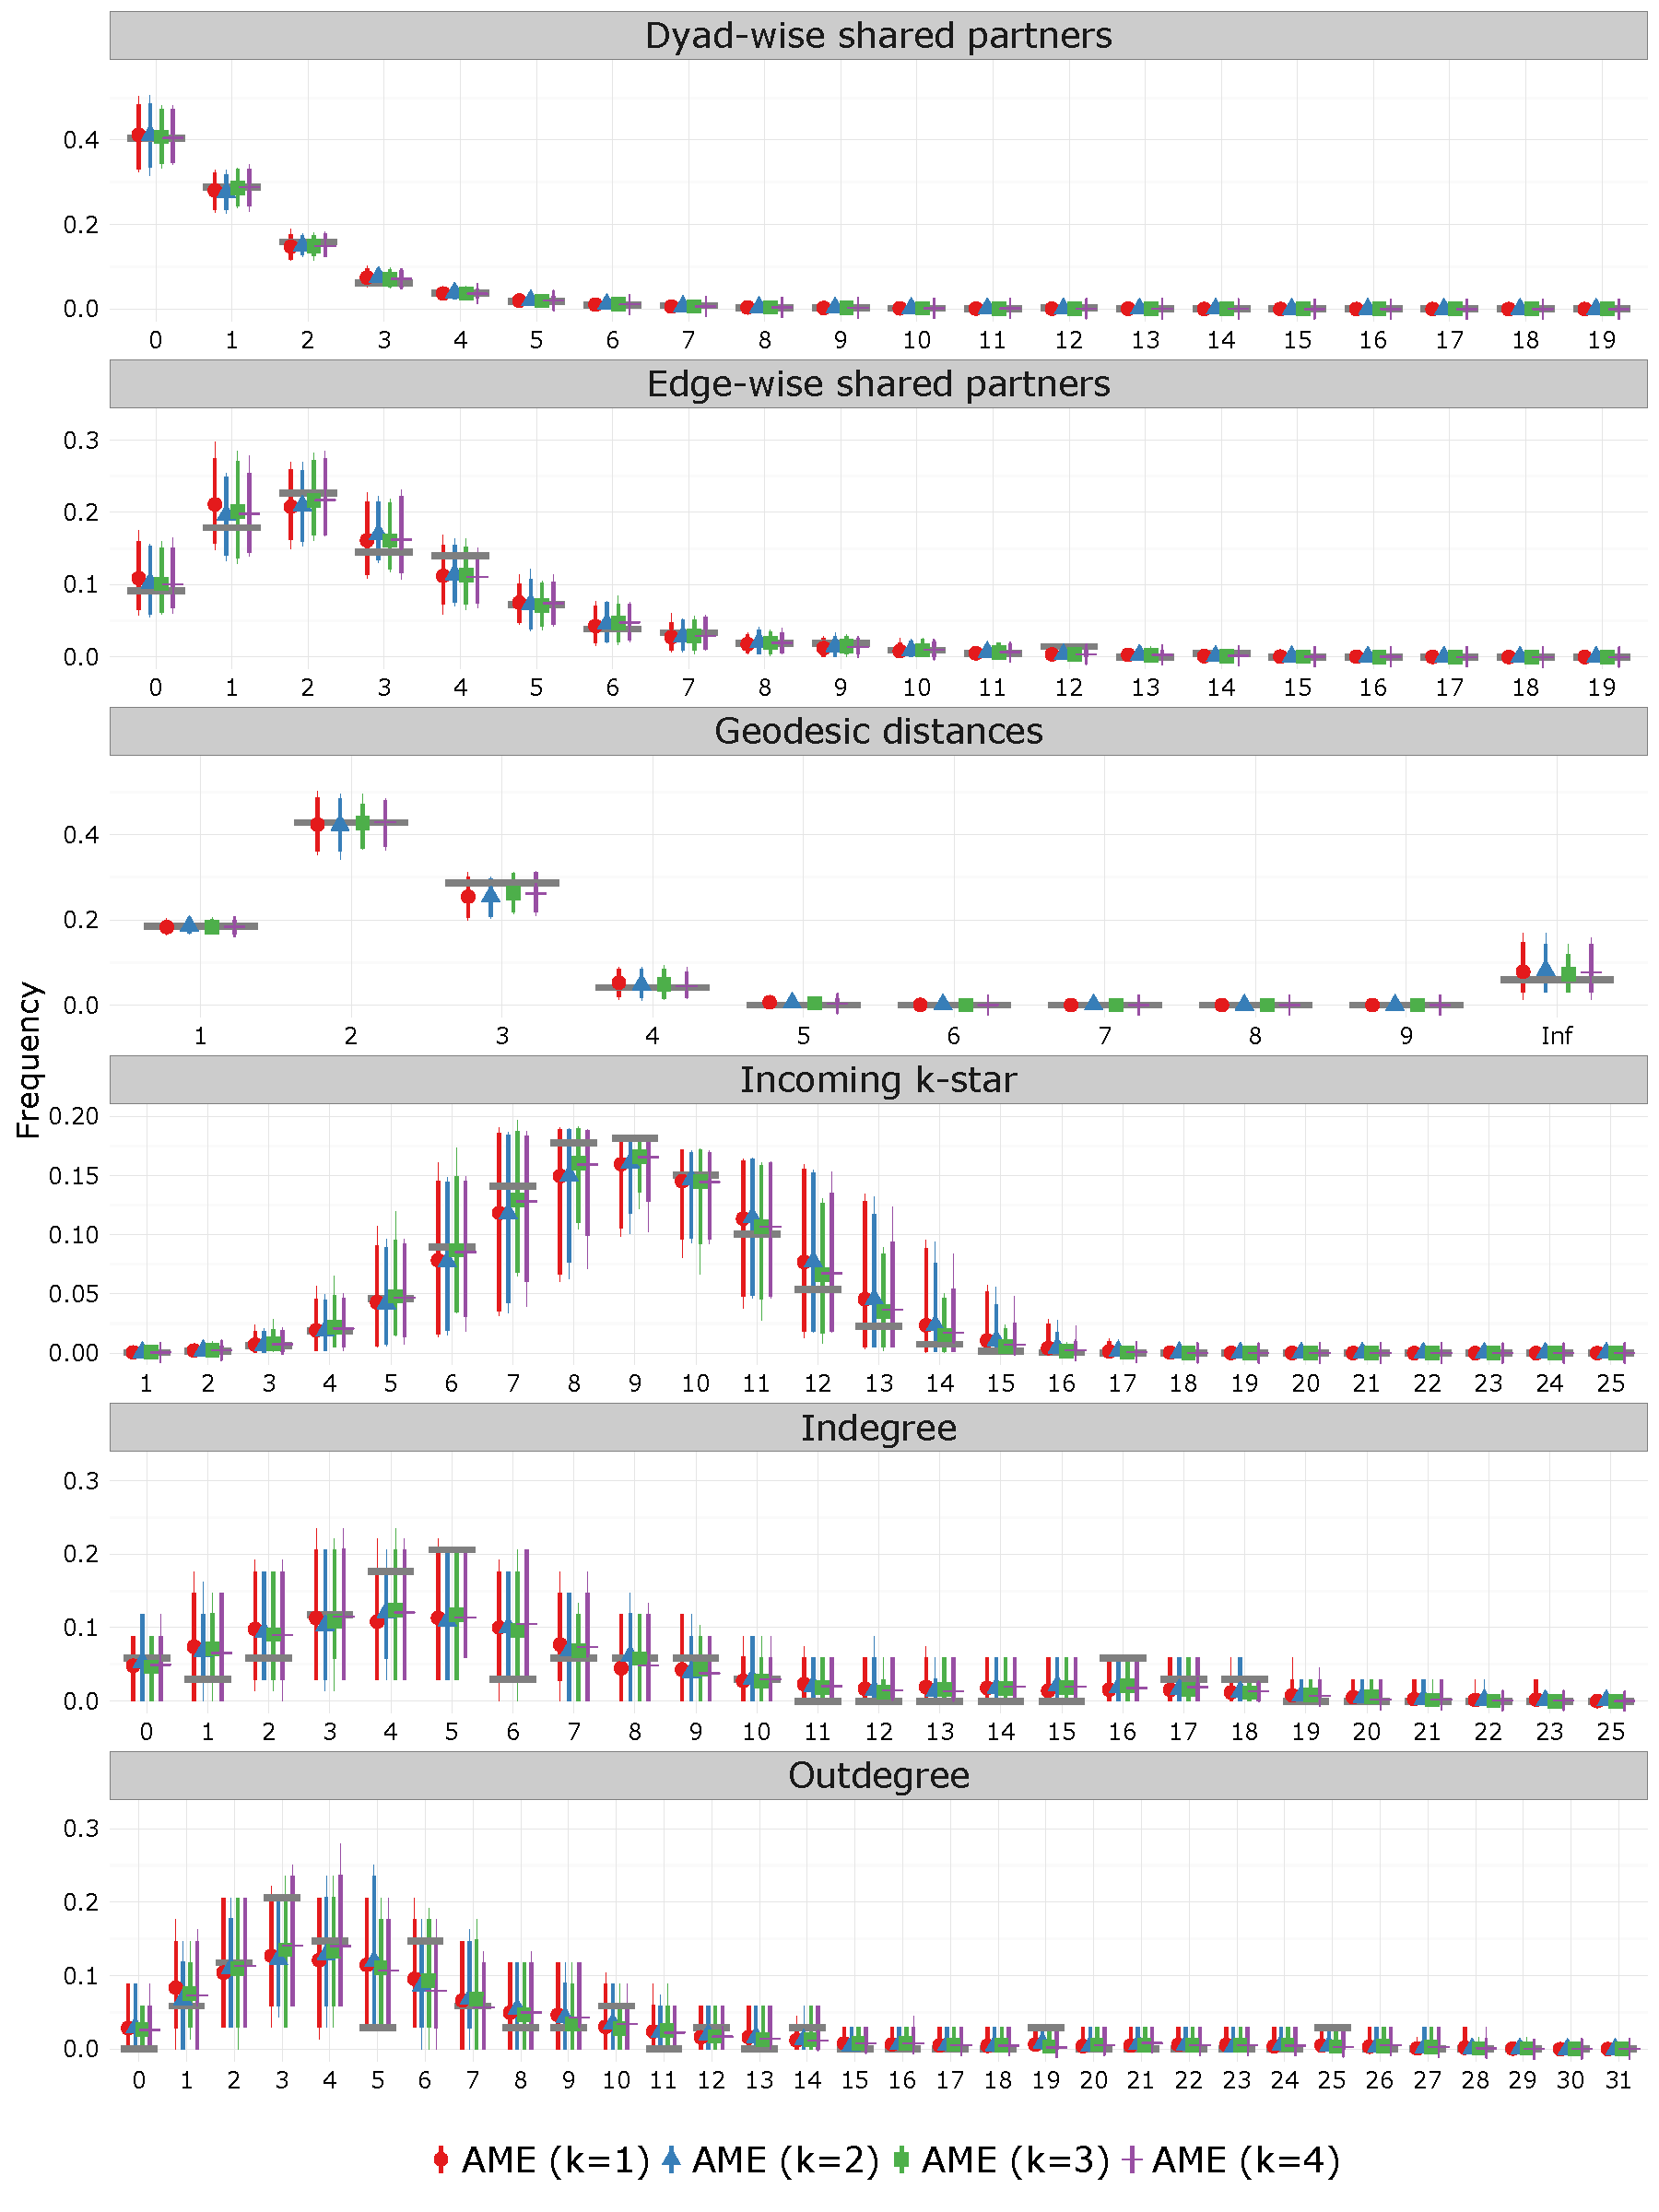
\includegraphics[width=1\textwidth]{ggGofAll_ameSR}
	\caption{network stats }
	\label{fig:gofAll_ameSR}
\end{figure}
\FloatBarrier

\newpage
\begin{figure}[ht]
	\centering
	\begin{tabular}{cc}
	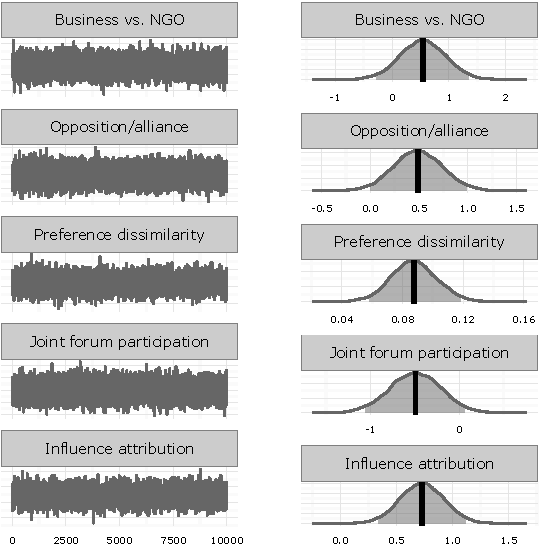
\includegraphics[width=.45\textwidth]{ameConv1_SR0} &
	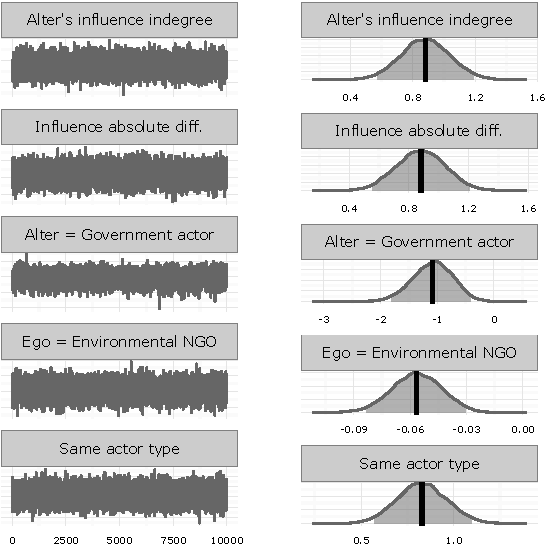
\includegraphics[width=.45\textwidth]{ameConv2_SR0}
	\end{tabular}
	\caption{ame convergence k = 0}
	\label{fig:ameConv}
\end{figure}

\begin{figure}[ht]
	\centering
	\begin{tabular}{cc}
	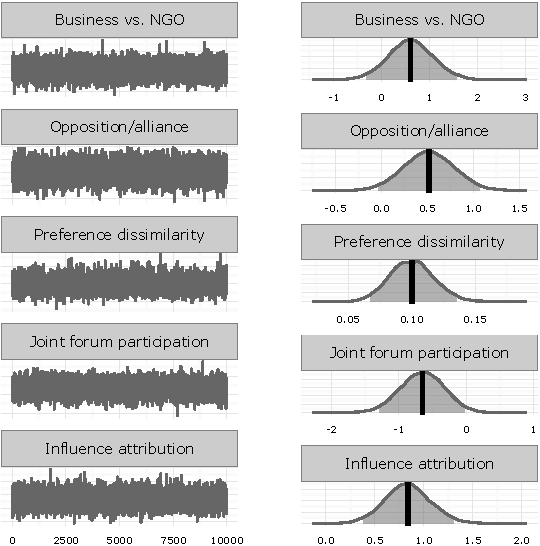
\includegraphics[width=.45\textwidth]{ameConv1_SR1} &
	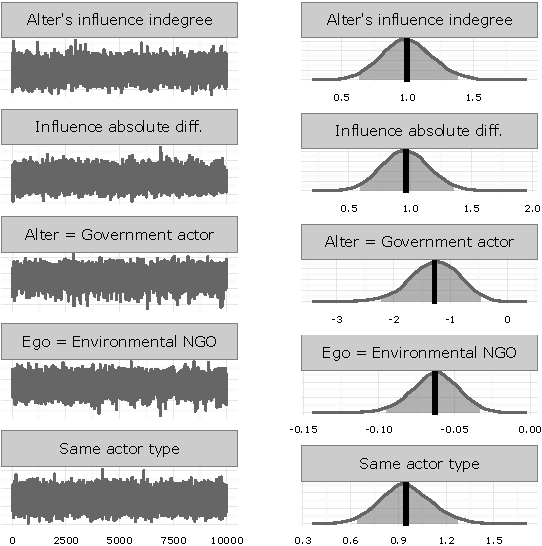
\includegraphics[width=.45\textwidth]{ameConv2_SR1}
	\end{tabular}
	\caption{ame convergence k=1}
	\label{fig:ameConv}
\end{figure}
\FloatBarrier
\newpage

\begin{figure}[ht]
	\centering
	\begin{tabular}{cc}
	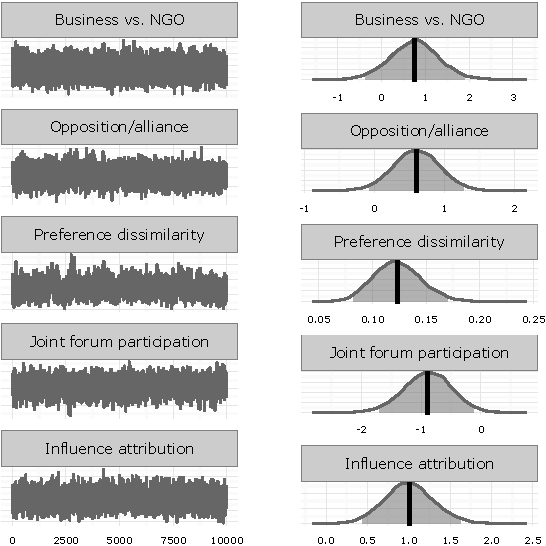
\includegraphics[width=.45\textwidth]{ameConv1_SR3} &
	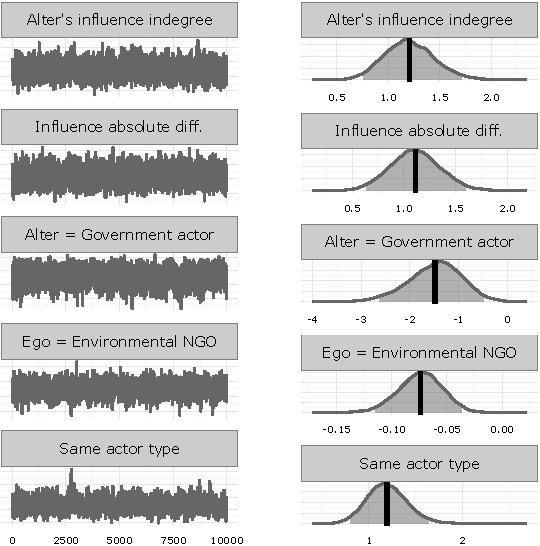
\includegraphics[width=.45\textwidth]{ameConv2_SR3}
	\end{tabular}
	\caption{ame convergence k=3}
	\label{fig:ameConv}
\end{figure}

\begin{figure}[ht]
	\centering
	\begin{tabular}{cc}
	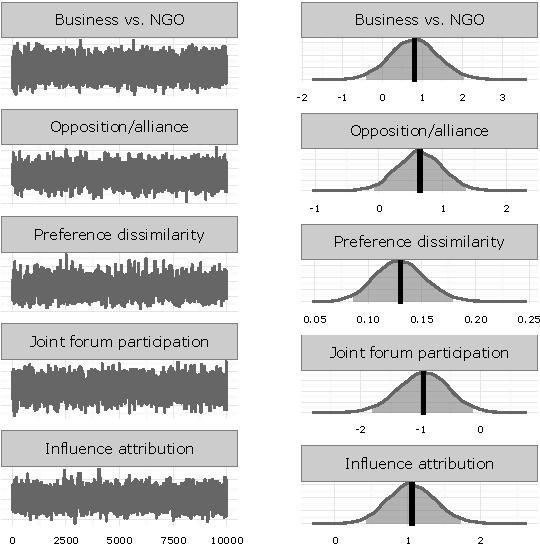
\includegraphics[width=.45\textwidth]{ameConv1_SR4} &
	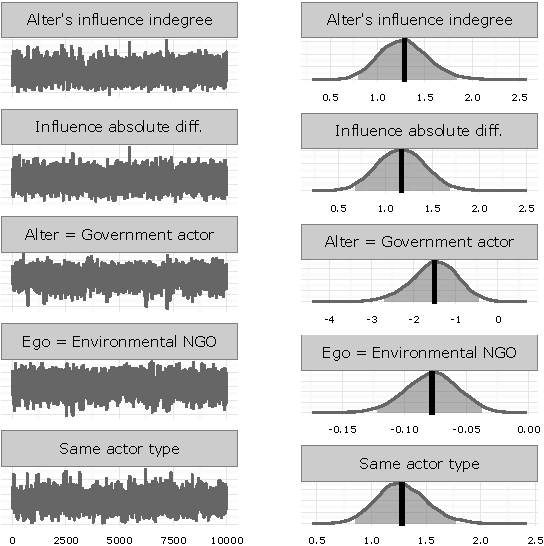
\includegraphics[width=.45\textwidth]{ameConv2_SR4}
	\end{tabular}
	\caption{ame convergence k = 4}
	\label{fig:ameConv}
\end{figure}
\FloatBarrier
\newpage

% % latex table generated in R 3.3.1 by xtable 1.8-2 package
% Sun Aug 21 03:38:29 2016
\begin{table}[ht]
\centering
\begingroup\tiny
\begin{tabular}{lccccc}
   & AME (k=0) & AME (k=1) & AME (k=2) & AME (k=3) & AME (k=4) \\ 
  \hline
\hline
Intercept/Edges & -2.19$^{\ast}$ & -2.72$^{\ast}$ & -2.75$^{\ast}$ & -2.92$^{\ast}$ & -3.03$^{\ast}$ \\ 
   & [-2.55; -1.85] & [-3.41; -1.82] & [-3.59; -1.88] & [-3.81; -2.04] & [-4.03; -1.99] \\ 
  \textbf{Conflicting policy preferences} &  &  &  &  &  \\ 
  $\;\;\;\;$ Business vs. NGO & -0.46 & -0.88$^{\ast}$ & -0.96$^{\ast}$ & -1.03$^{\ast}$ & -1.12$^{\ast}$ \\ 
   & [-0.95; -0.01] & [-1.64; -0.22] & [-1.86; -0.22] & [-1.96; -0.24] & [-2.15; -0.25] \\ 
  $\;\;\;\;$ Opposition/alliance & 0.65$^{\ast}$ & 0.79$^{\ast}$ & 0.86$^{\ast}$ & 0.95$^{\ast}$ & 1.03$^{\ast}$ \\ 
   & [0.44; 0.86] & [0.53; 1.07] & [0.56; 1.16] & [0.62; 1.32] & [0.67; 1.42] \\ 
  $\;\;\;\;$ Preference dissimilarity & -0.52$^{\ast}$ & -0.49 & -0.57 & -0.65 & -0.75$^{\ast}$ \\ 
   & [-0.95; -0.10] & [-1.03; 0.04] & [-1.17; 0.02] & [-1.34; 0.00] & [-1.47; -0.07] \\ 
  \textbf{Transaction costs} &  &  &  &  &  \\ 
  $\;\;\;\;$ Joint forum participation & 0.49$^{\ast}$ & 0.68$^{\ast}$ & 0.72$^{\ast}$ & 0.77$^{\ast}$ & 0.81$^{\ast}$ \\ 
   & [0.18; 0.79] & [0.30; 1.06] & [0.30; 1.13] & [0.30; 1.24] & [0.31; 1.32] \\ 
  \textbf{Influence} &  &  &  &  &  \\ 
  $\;\;\;\;$ Influence attribution & 0.76$^{\ast}$ & 0.86$^{\ast}$ & 0.93$^{\ast}$ & 1.01$^{\ast}$ & 1.08$^{\ast}$ \\ 
   & [0.52; 0.99] & [0.56; 1.16] & [0.59; 1.29] & [0.64; 1.41] & [0.68; 1.52] \\ 
  $\;\;\;\;$ Alter's influence indegree & 0.06$^{\ast}$ & 0.08$^{\ast}$ & 0.08$^{\ast}$ & 0.09$^{\ast}$ & 0.10$^{\ast}$ \\ 
   & [0.04; 0.08] & [0.05; 0.10] & [0.05; 0.11] & [0.06; 0.12] & [0.06; 0.14] \\ 
  $\;\;\;\;$ Influence absolute diff. & -0.03$^{\ast}$ & -0.04$^{\ast}$ & -0.05$^{\ast}$ & -0.05$^{\ast}$ & -0.06$^{\ast}$ \\ 
   & [-0.05; -0.01] & [-0.07; -0.02] & [-0.08; -0.02] & [-0.09; -0.02] & [-0.09; -0.02] \\ 
  $\;\;\;\;$ Alter = Government actor & 0.38$^{\ast}$ & 0.51$^{\ast}$ & 0.56$^{\ast}$ & 0.62$^{\ast}$ & 0.67$^{\ast}$ \\ 
   & [0.10; 0.64] & [0.13; 0.88] & [0.11; 1.01] & [0.13; 1.14] & [0.10; 1.27] \\ 
  \textbf{Functional requirements} &  &  &  &  &  \\ 
  $\;\;\;\;$ Ego = Environmental NGO & 0.49$^{\ast}$ & 0.50 & 0.54 & 0.61 & 0.72 \\ 
   & [0.22; 0.77] & [-0.24; 1.18] & [-0.27; 1.32] & [-0.31; 1.50] & [-0.27; 1.78] \\ 
  $\;\;\;\;$ Same actor type & 0.74$^{\ast}$ & 0.89$^{\ast}$ & 0.93$^{\ast}$ & 0.98$^{\ast}$ & 1.02$^{\ast}$ \\ 
   & [0.49; 1.00] & [0.58; 1.21] & [0.58; 1.28] & [0.60; 1.36] & [0.62; 1.45] \\ 
   \hline
\hline
\end{tabular}
\endgroup
\caption{* p $<$ 0.05 (or 0 outside the 95\% confidence interval).} 
\label{tab:regTable_latSpace}
\end{table}

% % latex table generated in R 3.3.1 by xtable 1.8-2 package
% Sun Aug 21 03:26:28 2016
\begin{table}[ht]
\centering
\begingroup\normalsize
\begin{tabular}{lcc}
  & AUC & AUC (PR) \\ 
  \hline
\hline
AME (k=4) & 0.99 & 0.95 \\ 
  AME (k=3) & 0.98 & 0.93 \\ 
  AME (k=2) & 0.97 & 0.89 \\ 
  AME (k=1) & 0.95 & 0.85 \\ 
  AME (k=0) & 0.87 & 0.66 \\ 
  \end{tabular}
\endgroup
\caption{Area under the curve (AUC) comparison for latent space approaches.} 
\label{tab:aucTable_latSpace}
\end{table}


% \begin{figure}[ht]
% 	\centering
% 	\begin{tabular}{cc}
% 	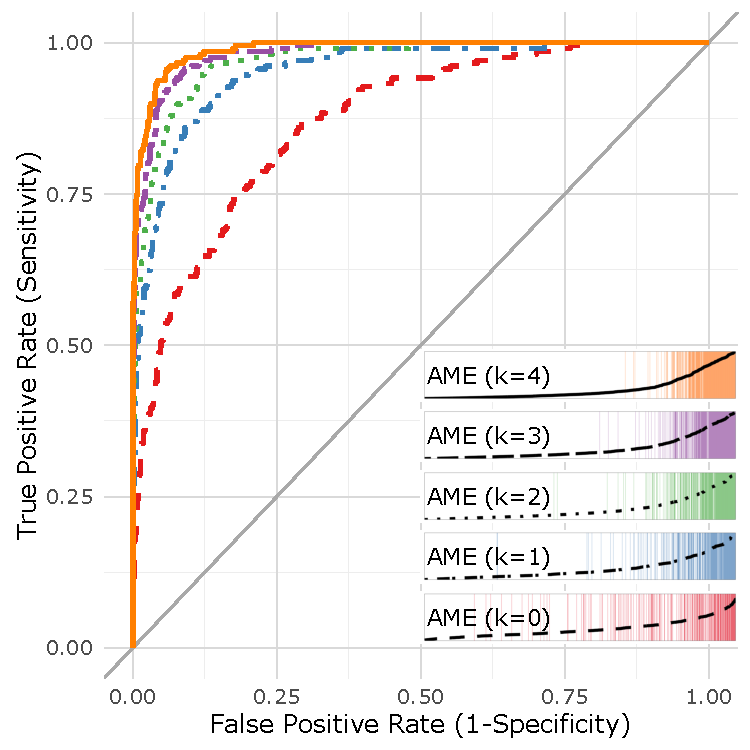
\includegraphics[width=.5\textwidth]{roc_ame} & 
% 	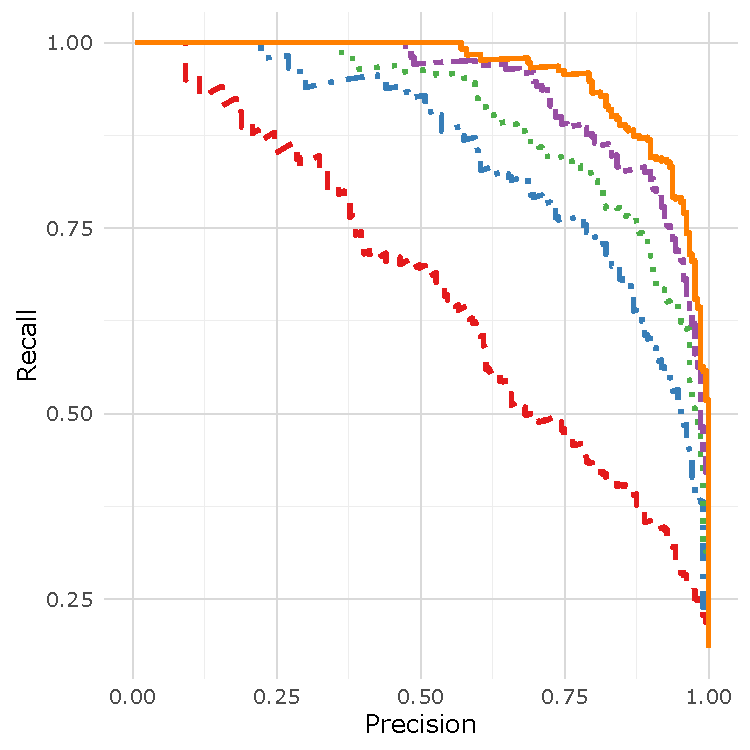
\includegraphics[width=.5\textwidth]{rocPr_ame}
% 	\end{tabular}
% 	\caption{ROC and separation plots}
% 	\label{fig:roc_latentSpace}
% \end{figure}

% \begin{figure}[ht]
% 	\centering
% 	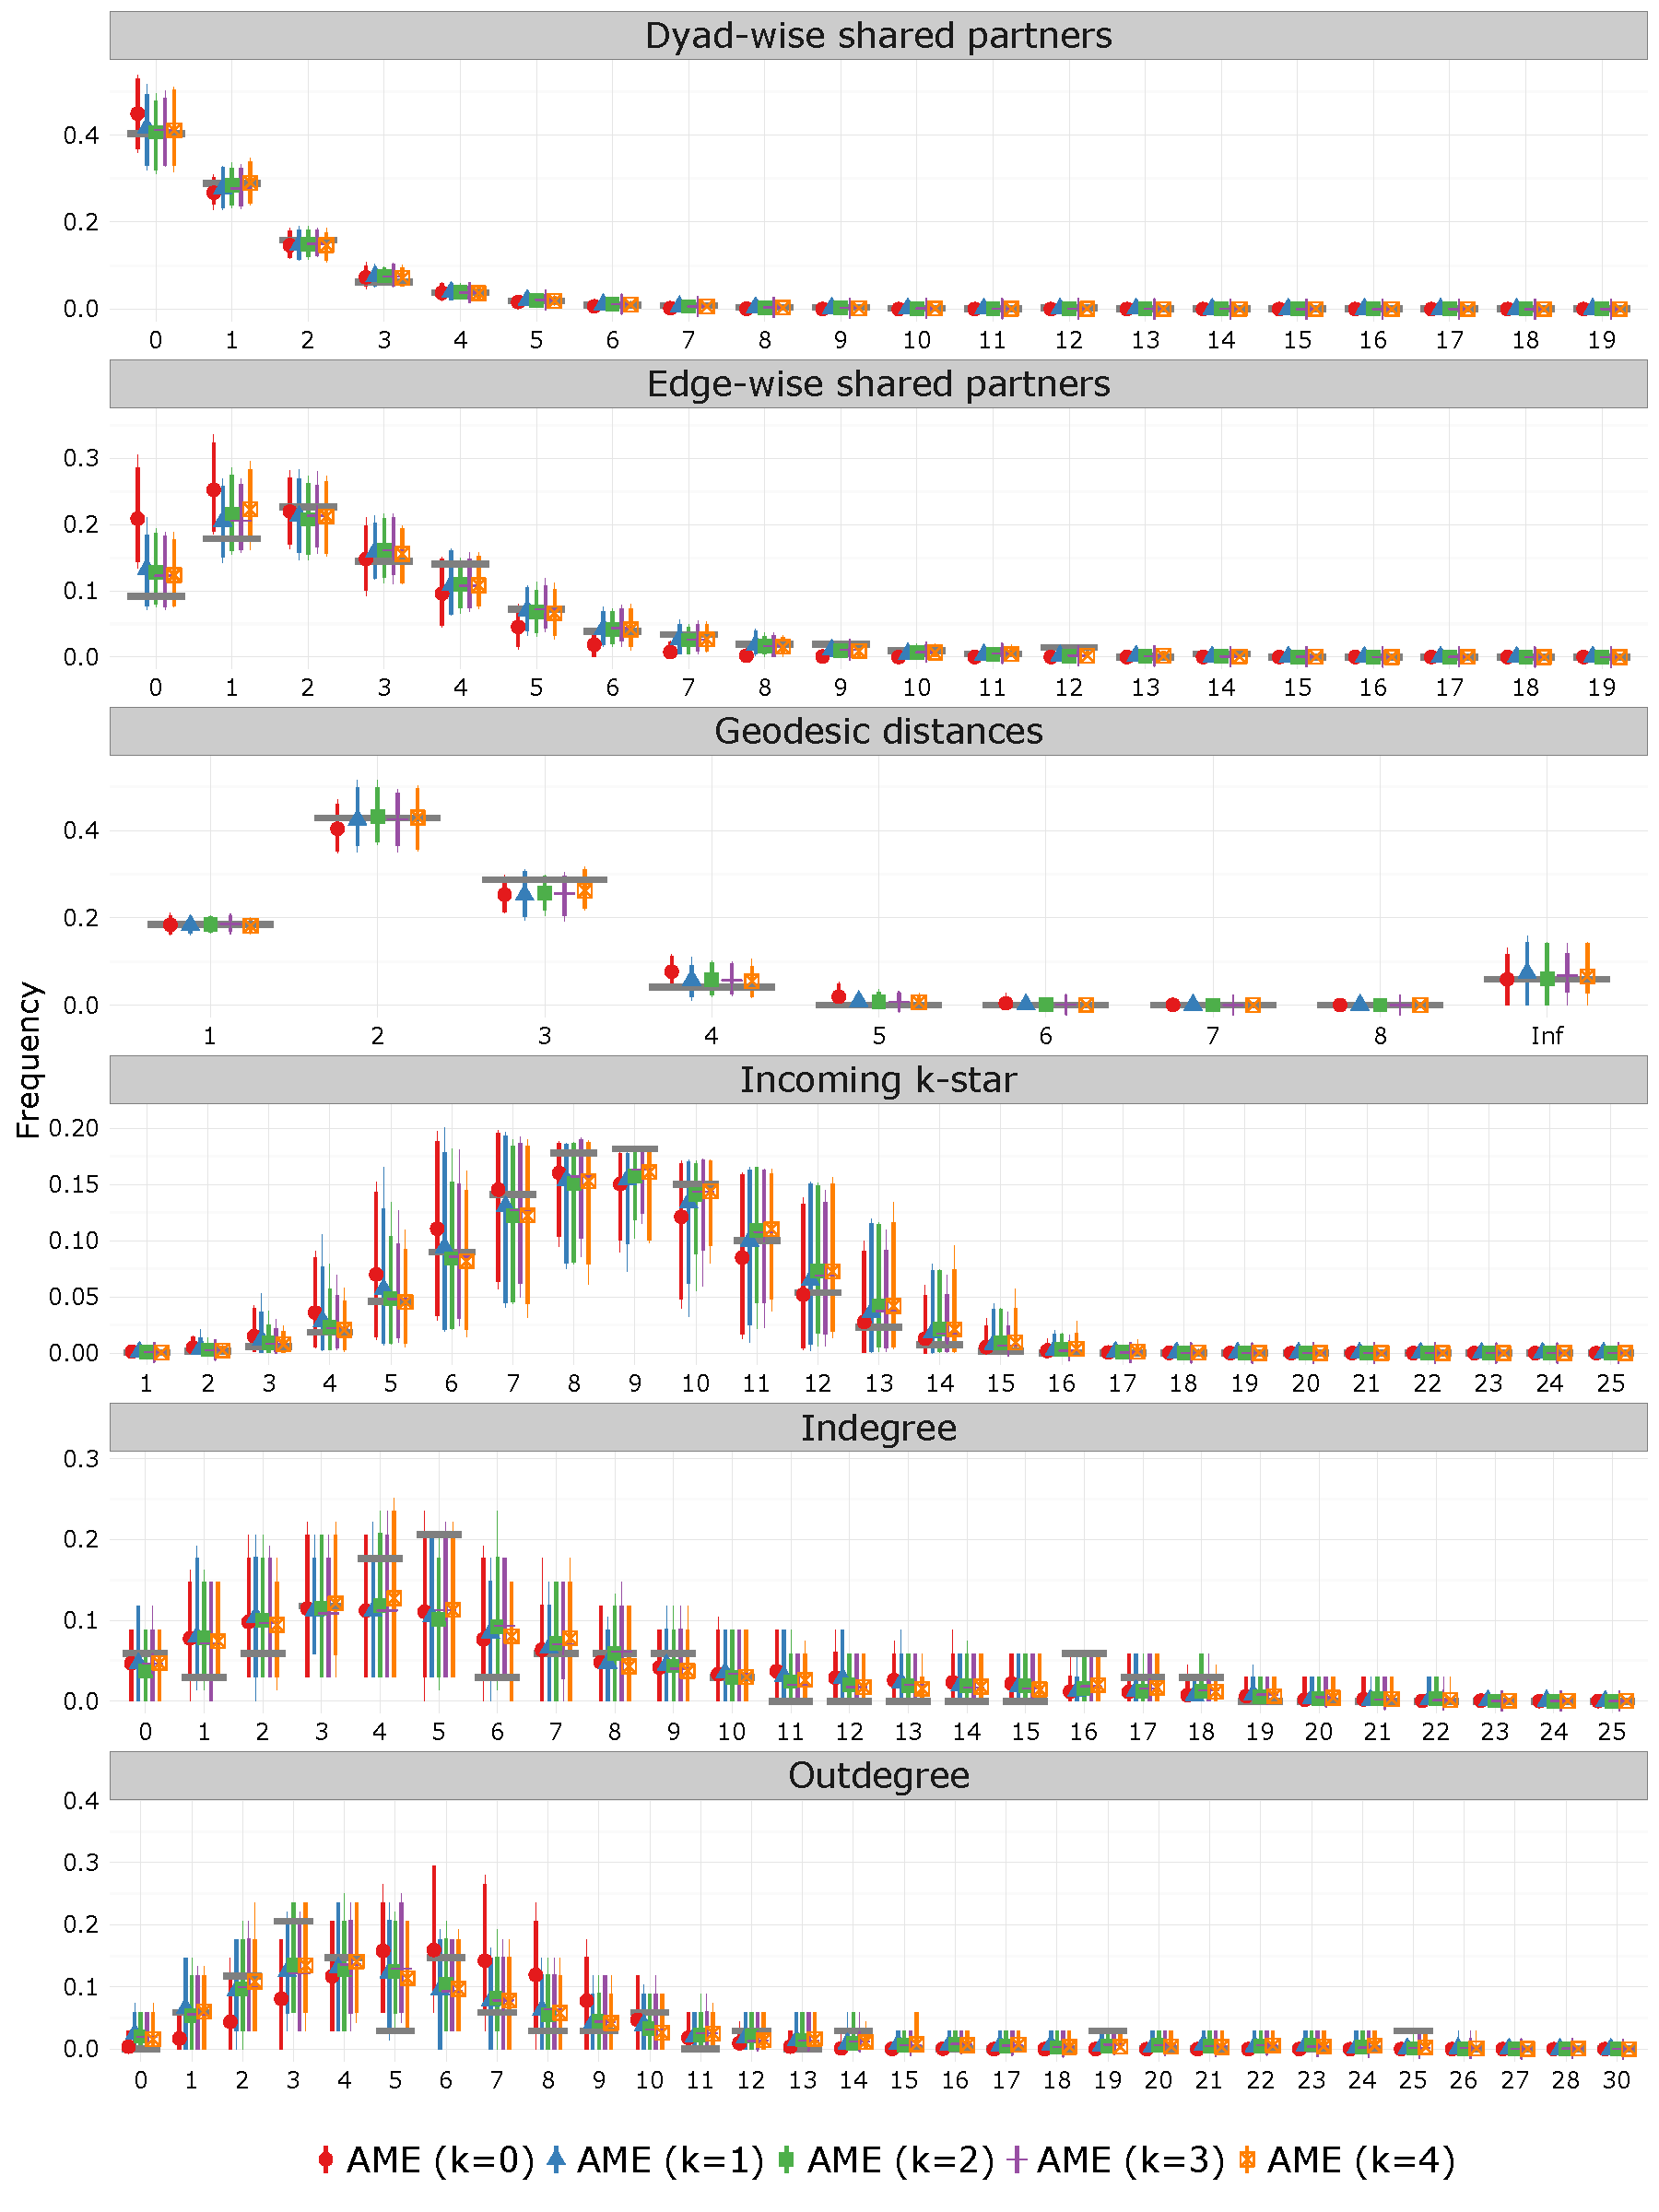
\includegraphics[width=1\textwidth]{ggGofAll_ame}
% 	\caption{network stats }
% 	\label{fig:gofAll_ame}
% \end{figure}

% \begin{figure}[ht]
% 	\centering
% 	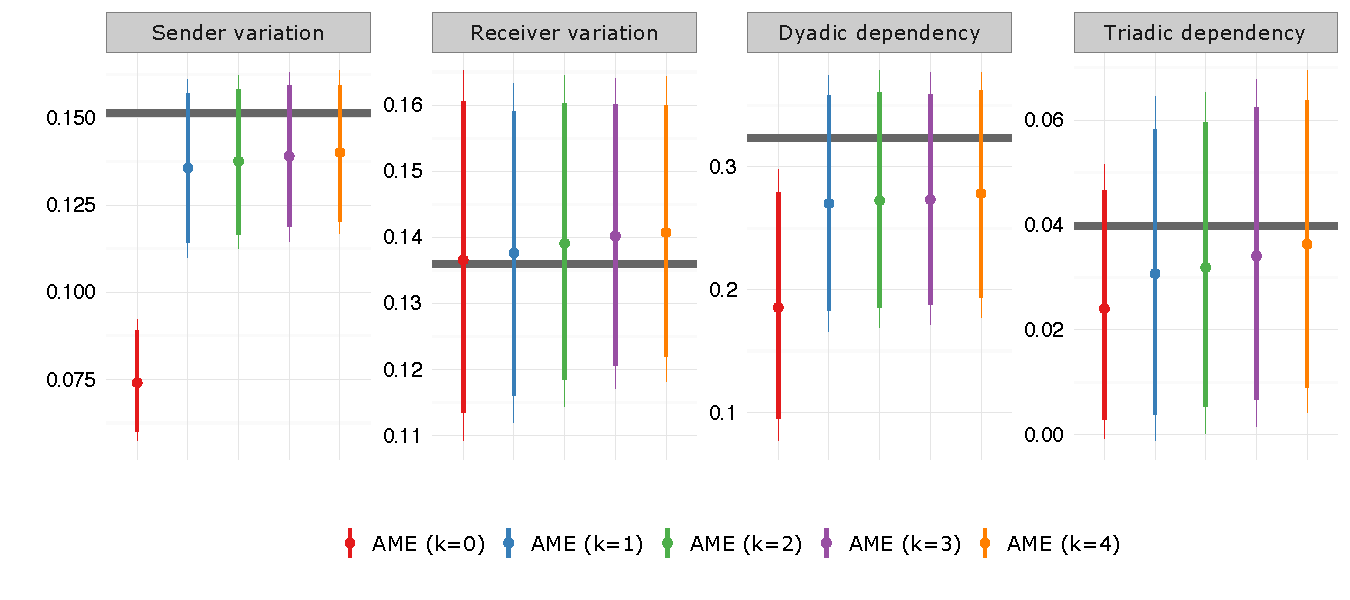
\includegraphics[width=1\textwidth]{netPerfCoef_ame}
% 	\caption{Posterior predictive goodness of fit summary}
% 	\label{fig:netPerfCoef_ame}
% \end{figure}

\newpage

% Bib stuff
\newpage
\bibliography{/Users/janus829/whistle/master, /Users/s7m/whistle/master}
% \bibliographystyle{/Users/janus829/Dropbox/bst/APSR}
\bibliographystyle{/Users/janus829/Dropbox/bst/jpr}
% \bibliographystyle{/Users/janus829/Dropbox/bst/ii}
\newpage

\end{document} 